%**************************************%
%*    Generated from PreTeXt source   *%
%*    on 2019-06-14T10:24:21-05:00    *%
%*                                    *%
%*   http://mathbook.pugetsound.edu   *%
%*                                    *%
%**************************************%
\documentclass[10pt,]{book}
%% Custom Preamble Entries, early (use latex.preamble.early)
%% Customized to load Palatino fonts
\usepackage[T1]{fontenc}
\renewcommand{\rmdefault}{zpltlf} %Roman font for use in math mode
\usepackage[scaled=.85]{beramono}% used only by \mathtt
\usepackage[type1]{cabin}%used only by \mathsf
\usepackage{amsmath,amssymb,amsthm}%load before newpxmath
\usepackage[varg,cmintegrals,bigdelims,varbb]{newpxmath}
\usepackage[scr=rsfso]{mathalfa}
\usepackage{bm} %load after all math to give access to bold math
% Now load the otf text fonts using fontspec--wont affect math
\usepackage[no-math]{fontspec}
\setmainfont{TeXGyrePagellaX}
\defaultfontfeatures{Ligatures=TeX,Scale=1,Mapping=tex-text}
\linespread{1.02}

%% Default LaTeX packages
%%   1.  always employed (or nearly so) for some purpose, or
%%   2.  a stylewriter may assume their presence
\usepackage{geometry}
%% Some aspects of the preamble are conditional,
%% the LaTeX engine is one such determinant
\usepackage{ifthen}
\usepackage{ifxetex,ifluatex}
%% Raster graphics inclusion
\usepackage{graphicx}
%% Colored boxes, and much more, though mostly styling
%% skins library provides "enhanced" skin, employing tikzpicture
%% boxes may be configured as "breakable" or "unbreakable"
\usepackage{tcolorbox}
\tcbuselibrary{skins}
\tcbuselibrary{breakable}
%% Hyperref should be here, but likes to be loaded late
%%
%% Inline math delimiters, \(, \), need to be robust
%% 2016-01-31:  latexrelease.sty  supersedes  fixltx2e.sty
%% If  latexrelease.sty  exists, bugfix is in kernel
%% If not, bugfix is in  fixltx2e.sty
%% See:  https://tug.org/TUGboat/tb36-3/tb114ltnews22.pdf
%% and read "Fewer fragile commands" in distribution's  latexchanges.pdf
\IfFileExists{latexrelease.sty}{}{\usepackage{fixltx2e}}
%% Text height identically 9 inches, text width varies on point size
%% See Bringhurst 2.1.1 on measure for recommendations
%% 75 characters per line (count spaces, punctuation) is target
%% which is the upper limit of Bringhurst's recommendations
\geometry{letterpaper,total={340pt,9.0in}}
%% Custom Page Layout Adjustments (use latex.geometry)
\geometry{paperwidth=7.44in,paperheight=9.69in,tmargin=.5in,bmargin=.3in,hmargin=.75in,bindingoffset=.4in,includeheadfoot }
%% This LaTeX file may be compiled with pdflatex, xelatex, or lualatex
%% The following provides engine-specific capabilities
%% Generally, xelatex and lualatex will do better languages other than US English
%% You can pick from the conditional if you will only ever use one engine
\ifthenelse{\boolean{xetex} \or \boolean{luatex}}{%
%% begin: xelatex and lualatex-specific configuration
%% fontspec package will make Latin Modern (lmodern) the default font
\ifxetex\usepackage{xltxtra}\fi
\usepackage{fontspec}
%% realscripts is the only part of xltxtra relevant to lualatex 
\ifluatex\usepackage{realscripts}\fi
%% 
%% Extensive support for other languages
\usepackage{polyglossia}
%% Main document language is US English
\setdefaultlanguage{english}
%% Spanish
\setotherlanguage{spanish}
%% Vietnamese
\setotherlanguage{vietnamese}
%% end: xelatex and lualatex-specific configuration
}{%
%% begin: pdflatex-specific configuration
%% translate common Unicode to their LaTeX equivalents
%% Also, fontenc with T1 makes CM-Super the default font
%% (\input{ix-utf8enc.dfu} from the "inputenx" package is possible addition (broken?)
\usepackage[T1]{fontenc}
\usepackage[utf8]{inputenc}
%% end: pdflatex-specific configuration
}
%% Monospace font: Inconsolata (zi4)
%% Sponsored by TUG: http://levien.com/type/myfonts/inconsolata.html
%% See package documentation for excellent instructions
%% One caveat, seem to need full file name to locate OTF files
%% Loads the "upquote" package as needed, so we don't have to
%% Upright quotes might come from the  textcomp  package, which we also use
%% We employ the shapely \ell to match Google Font version
%% pdflatex: "varqu" option produces best upright quotes
%% xelatex,lualatex: add StylisticSet 1 for shapely \ell
%% xelatex,lualatex: add StylisticSet 2 for plain zero
%% xelatex,lualatex: we add StylisticSet 3 for upright quotes
%% 
\ifthenelse{\boolean{xetex} \or \boolean{luatex}}{%
%% begin: xelatex and lualatex-specific monospace font
\usepackage{zi4}
\setmonofont[BoldFont=Inconsolatazi4-Bold.otf,StylisticSet={1,3}]{Inconsolatazi4-Regular.otf}
%% end: xelatex and lualatex-specific monospace font
}{%
%% begin: pdflatex-specific monospace font
%% "varqu" option provides textcomp \textquotedbl glyph
%% "varl"  option provides shapely "ell"
\usepackage[varqu,varl]{zi4}
%% end: pdflatex-specific monospace font
}
%% \mono macro for content of "c" element only
\newcommand{\mono}[1]{\texttt{#1}}
%% Symbols, align environment, bracket-matrix
\usepackage{amsmath}
\usepackage{amssymb}
%% allow page breaks within display mathematics anywhere
%% level 4 is maximally permissive
%% this is exactly the opposite of AMSmath package philosophy
%% there are per-display, and per-equation options to control this
%% split, aligned, gathered, and alignedat are not affected
\allowdisplaybreaks[4]
%% allow more columns to a matrix
%% can make this even bigger by overriding with  latex.preamble.late  processing option
\setcounter{MaxMatrixCols}{30}
%%
%% Color support, xcolor package
%% Always loaded, for: add/delete text, author tools
\PassOptionsToPackage{usenames,dvipsnames,svgnames,table}{xcolor}
\usepackage{xcolor}
%%
%% Semantic Macros
%% To preserve meaning in a LaTeX file
%% Only defined here if required in this document
%% Used for inline definitions of terms
\newcommand{\terminology}[1]{\textbf{#1}}
%% Used for fillin answer blank
%% Argument is length in em
\newcommand{\fillin}[1]{\underline{\hspace{#1em}}}
%% Used to markup initialisms, text or titles
%% default is small caps (Bringhurst, 4e, 3.2.2, p. 48)
%% Titles are no-ops now, see comments in XSL source
\newcommand{\initialism}[1]{\textsc{\MakeLowercase{#1}}}
\DeclareRobustCommand{\initialismintitle}[1]{\texorpdfstring{#1}{#1}}
%% Subdivision Numbering, Chapters, Sections, Subsections, etc
%% Subdivision numbers may be turned off at some level ("depth")
%% A section *always* has depth 1, contrary to us counting from the document root
%% The latex default is 3.  If a larger number is present here, then
%% removing this command may make some cross-references ambiguous
%% The precursor variable $numbering-maxlevel is checked for consistency in the common XSL file
\setcounter{secnumdepth}{3}
%% Environments with amsthm package
%% Theorem-like environments in "plain" style, with or without proof
\usepackage{amsthm}
\theoremstyle{plain}
%% Numbering for Theorems, Conjectures, Examples, Figures, etc
%% Controlled by  numbering.theorems.level  processing parameter
%% Always need a theorem environment to set base numbering scheme
%% even if document has no theorems (but has other environments)
\newtheorem{theorem}{Theorem}[section]
%% Only variants actually used in document appear here
%% Style is like a theorem, and for statements without proofs
%% Numbering: all theorem-like numbered consecutively
%% i.e. Corollary 4.3 follows Theorem 4.2
%% Definition-like environments, normal text
%% Numbering is in sync with theorems, etc
\theoremstyle{definition}
\newtheorem{definition}[theorem]{Definition}
%% Remark-like environments, normal text
%% Numbering is in sync with theorems, etc
\theoremstyle{definition}
\newtheorem{remark}[theorem]{Remark}
\newtheorem{note}[theorem]{Note}
\newtheorem{warning}[theorem]{Warning}
%% Example-like environments, normal text
%% Numbering is in sync with theorems, etc
\theoremstyle{definition}
\newtheorem{example}[theorem]{Example}
%% begin: assemblage
%% minimally structured content, high visibility presentation
%% One optional argument (title) with default value blank
%% 3mm space below dropped title is increase over 2mm default
\newtcolorbox{assemblage}[1][]
  {breakable, skin=enhanced, arc=2ex, colback=blue!5, colframe=blue!75!black,
   colbacktitle=blue!20, coltitle=black, boxed title style={sharp corners, frame hidden},
   fonttitle=\bfseries, attach boxed title to top left={xshift=4mm,yshift=-3mm}, top=3mm, title={#1}}
%% end: assemblage
%% objectives: early in a subdivision, introduction/list/conclusion
%% objectives environment and style
\newenvironment{objectives}[1]{\noindent\rule{\linewidth}{0.1ex}\newline{\textbf{{\large#1}}\par\smallskip}}{\par\noindent\rule{\linewidth}{0.1ex}\par\smallskip}
%% Numbering for inline exercises is in sync with theorems, normal text
\theoremstyle{definition}
\newtheorem{exercise}[theorem]{Exercise}
%% Localize LaTeX supplied names (possibly none)
\renewcommand*{\appendixname}{Appendix}
\renewcommand*{\chaptername}{Chapter}
%% Equation Numbering
%% Controlled by  numbering.equations.level  processing parameter
\numberwithin{equation}{section}
%% For improved tables
\usepackage{array}
%% Some extra height on each row is desirable, especially with horizontal rules
%% Increment determined experimentally
\setlength{\extrarowheight}{0.2ex}
%% Define variable thickness horizontal rules, full and partial
%% Thicknesses are 0.03, 0.05, 0.08 in the  booktabs  package
\makeatletter
\newcommand{\hrulethin}  {\noalign{\hrule height 0.04em}}
\newcommand{\hrulemedium}{\noalign{\hrule height 0.07em}}
\newcommand{\hrulethick} {\noalign{\hrule height 0.11em}}
% TeX imported from a WeBWorK server might use booktabs rule commands
% Replace/delete these three approximations if booktabs is loaded
\newcommand{\toprule}{\hrulethick}
\newcommand{\midrule}{\hrulemedium}
\newcommand{\bottomrule}{\hrulethick}
%% We preserve a copy of the \setlength package before other
%% packages (extpfeil) get a chance to load packages that redefine it
\let\oldsetlength\setlength
\newlength{\Oldarrayrulewidth}
\newcommand{\crulethin}[1]%
{\noalign{\global\oldsetlength{\Oldarrayrulewidth}{\arrayrulewidth}}%
\noalign{\global\oldsetlength{\arrayrulewidth}{0.04em}}\cline{#1}%
\noalign{\global\oldsetlength{\arrayrulewidth}{\Oldarrayrulewidth}}}%
\newcommand{\crulemedium}[1]%
{\noalign{\global\oldsetlength{\Oldarrayrulewidth}{\arrayrulewidth}}%
\noalign{\global\oldsetlength{\arrayrulewidth}{0.07em}}\cline{#1}%
\noalign{\global\oldsetlength{\arrayrulewidth}{\Oldarrayrulewidth}}}
\newcommand{\crulethick}[1]%
{\noalign{\global\oldsetlength{\Oldarrayrulewidth}{\arrayrulewidth}}%
\noalign{\global\oldsetlength{\arrayrulewidth}{0.11em}}\cline{#1}%
\noalign{\global\oldsetlength{\arrayrulewidth}{\Oldarrayrulewidth}}}
%% Single letter column specifiers defined via array package
\newcolumntype{A}{!{\vrule width 0.04em}}
\newcolumntype{B}{!{\vrule width 0.07em}}
\newcolumntype{C}{!{\vrule width 0.11em}}
\makeatother
\newcommand{\tablecelllines}[3]%
{\begin{tabular}[#2]{@{}#1@{}}#3\end{tabular}}
%% Figures, Tables, Listings, Named Lists, Floats
%% The [H]ere option of the float package fixes floats in-place,
%% in deference to web usage, where floats are totally irrelevant
%% You can remove some of this setup, to restore standard LaTeX behavior
%% HOWEVER, numbering of figures/tables AND theorems/examples/remarks, etc
%% may de-synchronize with the numbering in the HTML version
%% You can remove the "placement={H}" option to allow flotation and
%% preserve numbering, BUT the numbering may then appear "out-of-order"
%% Floating environments: http://tex.stackexchange.com/questions/95631/
\usepackage{float}
\usepackage{newfloat}
\usepackage{caption}%% Adjust stock figure environment so that it no longer floats
\SetupFloatingEnvironment{figure}{fileext=lof,placement={H},within=section,name=Figure}
\captionsetup[figure]{labelfont=bf}
%% http://tex.stackexchange.com/questions/16195
\makeatletter
\let\c@figure\c@theorem
\makeatother
%% Adjust stock table environment so that it no longer floats
\SetupFloatingEnvironment{table}{fileext=lot,placement={H},within=section,name=Table}
\captionsetup[table]{labelfont=bf}
%% http://tex.stackexchange.com/questions/16195
\makeatletter
\let\c@table\c@theorem
\makeatother
%% Footnote Numbering
%% We reset the footnote counter, as given by numbering.footnotes.level
\makeatletter\@addtoreset{footnote}{section}\makeatother
%% Multiple column, column-major lists
\usepackage{multicol}
%% More flexible list management, esp. for references and exercises
%% But also for specifying labels (i.e. custom order) on nested lists
\usepackage{enumitem}
%% Lists of exercises in their own section, maximum depth 4
\newlist{exerciselist}{description}{4}
\setlist[exerciselist]{leftmargin=0pt,itemsep=1.0ex,topsep=1.0ex,partopsep=0pt,parsep=0pt}
%% Support for index creation
%% imakeidx package does not require extra pass (as with makeidx)
%% Title of the "Index" section set via a keyword
%% Language support for the "see" and "see also" phrases
\usepackage{imakeidx}
\makeindex[title=Index, intoc=true]
\renewcommand{\seename}{see}
\renewcommand{\alsoname}{see also}
%% Package for breakable boxes on WeBWorK problems from server LaTeX
\usepackage{mdframed}
%% WeBWorK problem style
\mdfdefinestyle{webwork-server}{framemethod=default, linewidth=2pt}
%% hyperref driver does not need to be specified, it will be detected
\usepackage{hyperref}
%% configure hyperref's  \url  to match listings' inline verbatim
\renewcommand\UrlFont{\small\ttfamily}
%% Hyperlinking active in PDFs, all links solid and blue
\hypersetup{colorlinks=true,linkcolor=blue,citecolor=blue,filecolor=blue,urlcolor=blue}
\hypersetup{pdftitle={Active Calculus}}
%% If you manually remove hyperref, leave in this next command
\providecommand\phantomsection{}
%% If tikz has been loaded, replace ampersand with \amp macro
%% NB: calc redefines \setlength
\usepackage{calc}
%% used repeatedly for vertical dimensions of sidebyside panels
\newlength{\panelmax}
%% extpfeil package for certain extensible arrows,
%% as also provided by MathJax extension of the same name
%% NB: this package loads mtools, which loads calc, which redefines
%%     \setlength, so it can be removed if it seems to be in the 
%%     way and your math does not use:
%%     
%%     \xtwoheadrightarrow, \xtwoheadleftarrow, \xmapsto, \xlongequal, \xtofrom
%%     
%%     we have had to be extra careful with variable thickness
%%     lines in tables, and so also load this package late
\usepackage{extpfeil}
%% Custom Preamble Entries, late (use latex.preamble.late)
%% Used to get WeBWorK logo into margin next to WW exercises
\usepackage{marginnote}
%%%%%%%%%%%%%%%%%%%%%%%%%%%%%%%%%%%%%%%%
% Modified from Mitch Keller's chapter handling 
%%%%%%%%%%%%%%%%%%%%%%%%%%%%%%%%%%%%%%%%
%%% This is from common
\definecolor{ActiveBlue}{cmyk}{1, 0.5, 0, 0.35}
\colorlet{chaptercolor}{ActiveBlue}
%%%%%%%%%%%%%%%%%%%%%%%%%%%%%%%%%%%%%%%%
% Basic paragraph parameters 
%%%%%%%%%%%%%%%%%%%%%%%%%%%%%%%%%%%%%%%%
\setlength{\parindent}{0mm}
\setlength{\parskip}{0.5pc}
%%%%%%%%%%%%%%%%%%%%%%%%%%%%%%%%%%%%%%%%
% In print, trying to reduce color use 
%%%%%%%%%%%%%%%%%%%%%%%%%%%%%%%%%%%%%%%%
\hypersetup{colorlinks=true,linkcolor=black,citecolor=black,filecolor=black,urlcolor=black}
%%%%%%%%%%%%%%%%%%%%%%%%%%%%%%%%%%%%%%%%
% Start sections on new page, just not the first one 
%%%%%%%%%%%%%%%%%%%%%%%%%%%%%%%%%%%%%%%%
\let\oldsection\section 
\renewcommand\section{\znewpage\oldsection}

\let\oldchapter\chapter 
\renewcommand\chapter{\clearpage\gdef\znewpage{\global\let\znewpage\clearpage}\oldchapter}

\global\let\znewpage\clearpage 

%% Begin: Author-provided packages
%% (From  docinfo/latex-preamble/package  elements)
%% End: Author-provided packages
%% Begin: Author-provided macros
%% (From  docinfo/macros  element)
%% Plus three from MBX for XML characters
\newcommand{\dollar}{\$}
\DeclareMathOperator{\erf}{erf}
\DeclareMathOperator{\arctanh}{arctanh}
\newcommand{\lt}{<}
\newcommand{\gt}{>}
\newcommand{\amp}{&}
%% End: Author-provided macros
%% PGML macros
%% formatted to exactly match output from PGML.pl as of 11/22/2016
%% but with some lines commented out
%\ifx\pgmlMarker\undefined
%  \newdimen\pgmlMarker \pgmlMarker=0.00314159pt  % hack to tell if \newline was used
%\fi
%\ifx\oldnewline\undefined \let\oldnewline=\newline \fi
%\def\newline{\oldnewline\hskip-\pgmlMarker\hskip\pgmlMarker\relax}%
%\parindent=0pt
%\catcode`\^^M=\active
%\def^^M{\ifmmode\else\fi\ignorespaces}%  skip paragraph breaks in the preamble
%\def\par{\ifmmode\else\endgraf\fi\ignorespaces}%
%\ifdim\lastskip=\pgmlMarker
%  \let\pgmlPar=\relax
% \else
  \let\pgmlPar=\par
%  \vadjust{\kern3pt}%
%\fi
%
%%%%%%%%%%%%%%%%%%%%%%%%%%%%%%%%%%%%%%%
%%
%%    definitions for PGML
%%
%
%\ifx\pgmlCount\undefined  % do not redefine if multiple files load PGML.pl
  \newcount\pgmlCount
  \newdimen\pgmlPercent
  \newdimen\pgmlPixels  \pgmlPixels=.5pt
%\fi
%\pgmlPercent=.01\hsize
%
\def\pgmlSetup{%
  \parskip=0pt \parindent=0pt
%  \ifdim\lastskip=\pgmlMarker\else\par\fi
  \pgmlPar
}%

\def\pgmlIndent{\par\advance\leftskip by 2em \advance\pgmlPercent by .02em \pgmlCount=0}%
\def\pgmlbulletItem{\par\indent\llap{$\bullet$ }\ignorespaces}%
\def\pgmlcircleItem{\par\indent\llap{$\circ$ }\ignorespaces}%
\def\pgmlsquareItem{\par\indent\llap{\vrule height 1ex width .75ex depth -.25ex\ }\ignorespaces}%
\def\pgmlnumericItem{\par\indent\advance\pgmlCount by 1 \llap{\the\pgmlCount. }\ignorespaces}%
\def\pgmlalphaItem{\par\indent{\advance\pgmlCount by `\a \llap{\char\pgmlCount. }}\advance\pgmlCount by 1\ignorespaces}%
\def\pgmlAlphaItem{\par\indent{\advance\pgmlCount by `\A \llap{\char\pgmlCount. }}\advance\pgmlCount by 1\ignorespaces}%
\def\pgmlromanItem{\par\indent\advance\pgmlCount by 1 \llap{\romannumeral\pgmlCount. }\ignorespaces}%
\def\pgmlRomanItem{\par\indent\advance\pgmlCount by 1 \llap{\uppercase\expandafter{\romannumeral\pgmlCount}. }\ignorespaces}%

\def\pgmlCenter{%
  \par \parfillskip=0pt
  \advance\leftskip by 0pt plus .5\hsize
  \advance\rightskip by 0pt plus .5\hsize
  \def\pgmlBreak{\break}%
}%
\def\pgmlRight{%
  \par \parfillskip=0pt
  \advance\leftskip by 0pt plus \hsize
  \def\pgmlBreak{\break}%
}%

\def\pgmlBreak{\\}%

\def\pgmlHeading#1{%
  \par\bfseries
  \ifcase#1 \or\huge \or\LARGE \or\large \or\normalsize \or\footnotesize \or\scriptsize \fi
}%

\def\pgmlRule#1#2{%
  \par\noindent
  \hbox{%
    \strut%
    \dimen1=\ht\strutbox%
    \advance\dimen1 by -#2%
    \divide\dimen1 by 2%
    \advance\dimen2 by -\dp\strutbox%
    \raise\dimen1\hbox{\vrule width #1 height #2 depth 0pt}%
  }%
  \par
}%

\def\pgmlIC#1{\futurelet\pgmlNext\pgmlCheckIC}%
\def\pgmlCheckIC{\ifx\pgmlNext\pgmlSpace \/\fi}%
{\def\getSpace#1{\global\let\pgmlSpace= }\getSpace{} }%
%
%{\catcode`\ =12\global\let\pgmlSpaceChar= }%
%{\obeylines\gdef\pgmlPreformatted{\par\small\ttfamily\hsize=10\hsize\obeyspaces\obeylines\let^^M=\pgmlNL\pgmlNL}}%
%\def\pgmlNL{\par\bgroup\catcode`\ =12\pgmlTestSpace}%
%\def\pgmlTestSpace{\futurelet\next\pgmlTestChar}%
%\def\pgmlTestChar{\ifx\next\pgmlSpaceChar\ \pgmlTestNext\fi\egroup}%
%\def\pgmlTestNext\fi\egroup#1{\fi\pgmlTestSpace}%
%
%\def^^M{\ifmmode\else\space\fi\ignorespaces}%
%% END PGML macros
%% Semantic macros for contributor list
\newcommand{\contributor}[1]{\parbox{\linewidth}{#1}\par\bigskip}
\newcommand{\contributorname}[1]{\textsc{#1}\\[0.25\baselineskip]}
\newcommand{\contributorinfo}[1]{\hspace*{0.05\linewidth}\parbox{0.95\linewidth}{\textsl{#1}}}
%% Title page information for book
\title{Active Calculus}
\author{Matthew Boelkins\\
Department of Mathematics\\
Grand Valley State University\\
\href{mailto:boelkinm@gvsu.edu}{\nolinkurl{boelkinm@gvsu.edu}}
}
\date{June 14, 2019}
\begin{document}
\frontmatter
%% begin: half-title
\thispagestyle{empty}
{\centering
\vspace*{0.28\textheight}
{\Huge Active Calculus}\\}
\clearpage
%% end:   half-title
%% begin: adcard
\thispagestyle{empty}
\null%
\clearpage
%% end:   adcard
%% begin: title page
%% Inspired by Peter Wilson's "titleDB" in "titlepages" CTAN package
\thispagestyle{empty}
{\centering
\vspace*{0.14\textheight}
%% Target for xref to top-level element is ToC
\addtocontents{toc}{\protect\hypertarget{index}{}}
{\Huge Active Calculus}\\[3\baselineskip]
{\Large Matthew Boelkins}\\[0.5\baselineskip]
{\Large Grand Valley State University}\\[3\baselineskip]
{\Large Contributing Authors}\\[0.5\baselineskip]
{\normalsize David Austin}\\[0.25\baselineskip]
Grand Valley State University\\[0.5\baselineskip]

{\normalsize Steven Schlicker}\\[0.25\baselineskip]
Grand Valley State University\\
[3\baselineskip]
{\Large Production Editor}\\[0.5\baselineskip]
{\normalsize Mitchel T. Keller}\\[0.25\baselineskip]
Morningside College\\
[3\baselineskip]
{\Large June 14, 2019}\\}
\clearpage
%% end:   title page
%% begin: copyright-page
\thispagestyle{empty}
\hypertarget{colophon-1}{}\vspace*{\stretch{2}}
\par\noindent
\textbf{Cover Photo}:\ \ James Haefner Photography
\par\vspace*{\stretch{2}}
\noindent{\bfseries Edition}: 2018\par\medskip
\noindent{\bfseries Website}: \href{http://activecalculus.org}{http://activecalculus.org}\par\medskip
\noindent\textcopyright\ 2012\textendash{}2018\quad{}Matthew Boelkins\\[0.5\baselineskip]
Permission is granted to copy and (re)distribute this material in any format and/or adapt it (even commercially) under the terms of the Creative Commons Attribution-ShareAlike 4.0 International License.  The work may be used for free in any way by any party so long as attribution is given to the author(s) and if the material is modified, the resulting contributions are distributed under the same license as this original.  All trademarks\texttrademark{} are the registered\textregistered{} marks of their respective owners. The graphic % group protects changes to lengths, releases boxes (?)
{% begin: group for a single side-by-side
% set panel max height to practical minimum, created in preamble
\setlength{\panelmax}{0pt}
\ifdefined\panelboxAimage\else\newsavebox{\panelboxAimage}\fi%
\begin{lrbox}{\panelboxAimage}
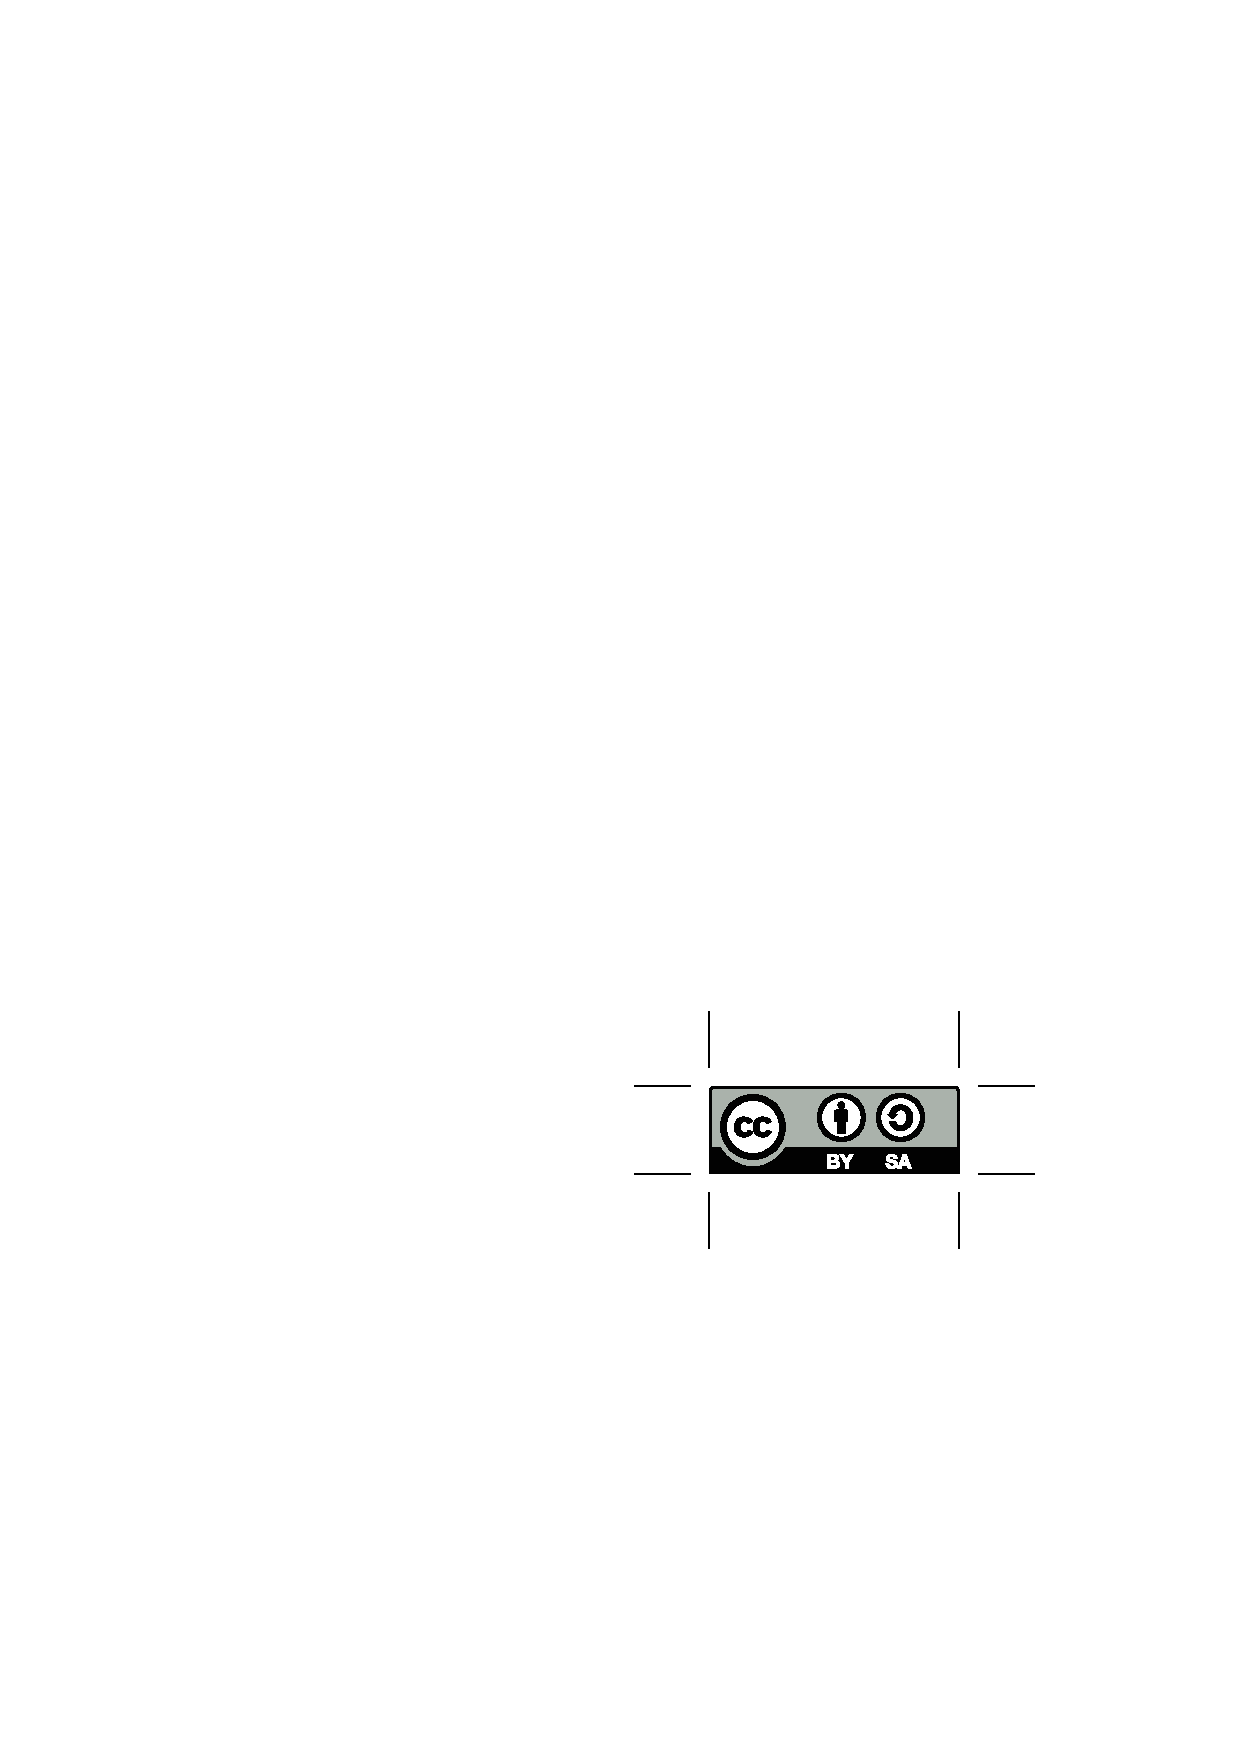
\includegraphics[width=0.25\linewidth]{images/CC-BY-SA-license}
\end{lrbox}
\ifdefined\phAimage\else\newlength{\phAimage}\fi%
\setlength{\phAimage}{\ht\panelboxAimage+\dp\panelboxAimage}
\settototalheight{\phAimage}{\usebox{\panelboxAimage}}
\setlength{\panelmax}{\maxof{\panelmax}{\phAimage}}
\leavevmode%
% begin: side-by-side as tabular
% \tabcolsep change local to group
\setlength{\tabcolsep}{0\linewidth}
% @{} suppress \tabcolsep at extremes, so margins behave as intended
\par\medskip\noindent
\hspace*{0.375\linewidth}%
\begin{tabular}{@{}*{1}{c}@{}}
\begin{minipage}[c][\panelmax][t]{0.25\linewidth}\usebox{\panelboxAimage}\end{minipage}\end{tabular}\\
% end: side-by-side as tabular
}% end: group for a single side-by-side
 that may appear in other locations in the text shows that the work is licensed with the Creative Commons and that the work may be used for free by any party so long as attribution is given to the author(s) and if the material is modified, the resulting contributions are distributed under the same license as this original. Full details may be found by visiting \href{https://creativecommons.org/licenses/by-sa/4.0/}{https://creativecommons.org/licenses/by-sa/4.0/}  or sending a letter to Creative Commons, 444 Castro Street, Suite 900, Mountain View, California, 94041, USA.\par\medskip
\vspace*{\stretch{1}}
\null\clearpage
%% end:   copyright-page
%% begin: acknowledgement
\chapter*{Acknowledgements}\label{acknowledgement-1}
\addcontentsline{toc}{chapter}{Acknowledgements}
\hypertarget{p-1}{}%
This text began as my sabbatical project in the winter semester of 2012, during which I wrote most of the material for the first four chapters. For the sabbatical leave, I am indebted to Grand Valley State University for its support of the project, as well as to my colleagues in the Department of Mathematics and the College of Liberal Arts and Sciences for their endorsement of the project. I'm also grateful to the American Institute of Mathematics for their \href{https://aimath.org/textbooks/}{support of free and open textbooks in general}, and their support of this one in particular.%
\par
\hypertarget{p-2}{}%
The beautiful full-color .eps graphics in the text are only possible because of David Austin of GVSU and Bill Casselman of the University of British Columbia. Building on their longstanding efforts to develop tools for high quality mathematical graphics, David wrote a library of Python routines that employ \href{http://gvsu.edu/s/bi}{Bill's PiScript program}; David's routines are so easy to use that even I could generate graphics like the professionals that he and Bill are. I am deeply grateful to them both.%
\par
\hypertarget{p-3}{}%
The current .html version of the text is possible only because of the amazing work of Rob Beezer and his development of the original \href{https://mathbook.pugetsound.edu}{Mathbook XML}, now known as PreTeXt. My ability to take advantage of Rob's work is due to the support of the American Institute of Mathematics, which funded me to attend a weeklong workshop in Mathbook XML in San Jose, CA, in April 2016, as well as the support of the ongoing \href{https://groups.google.com/forum/\#!forum/pretext-support}{user group}. David Farmer's conversion script saved me hundreds of hours of work by taking my original \LaTeX{} source and converting it to PreTeXt; David remains a major source of ongoing support and advocacy. Alex Jordan of Portland Community College has also been a tremendous help, and it is through Alex's fantastic work that live WeBWorK exercises are not only possible, but also included from the 2017 version forward. Mitch Keller of Morningside College agreed in early 2018 to serve as the book's production editor; his technical expertise has contributed to many aspects of the book, including the presence of answers to activities and non- WeBWorK exercises and other supporting material for instructors.%
\par
\hypertarget{p-4}{}%
For the 2018 edition, Kathy Yoshiwara of the AIM Editorial Board read the entire text and contributed editorial suggestions for every section. In short, she made the prose cleaner, more direct, and simply better. I'm deeply thankful for her time, effort, and insights.%
\par
\hypertarget{p-5}{}%
Over my more than 20 years at GVSU, many of my colleagues have shared with me ideas and resources for teaching calculus. I am particularly indebted to David Austin, Will Dickinson, Paul Fishback, Jon Hodge, and Steve Schlicker for their contributions that improved my teaching of and thinking about calculus, including materials that I have modified and used over many different semesters with students. Parts of these ideas can be found throughout this text. In addition, Will Dickinson and Steve Schlicker provided me access to a large number of their electronic notes and activities from teaching of differential and integral calculus, and those ideas and materials have similarly impacted my work and writing in positive ways, with some of their problems and approaches finding parallel presentation here.%
\par
\hypertarget{p-6}{}%
In the summer of 2012, David and Steve each agreed to write a chapter to support the completion of the material on integral calculus. David is the lead author of \hyperref[C-7]{Chapter~\ref{C-7}} and Steve the lead author of \hyperref[C-8]{Chapter~\ref{C-8}}. Along with our colleague Ted Sundstrom, Steve has also contributed a large number of problem and activity solutions and answers. I'm deeply grateful for how the work of these friends and colleagues has made the text so much better.%
\par
\hypertarget{p-7}{}%
Shelly Smith of GVSU and Matt Delong of Marian University both provided extensive comments on the first few chapters of early drafts, feedback that was immensely helpful in improving the text. As more and more people use the text, I am grateful to everyone who reads, edits, and uses this book, and hence contributes to its improvement through ongoing discussion.%
\par
\hypertarget{p-8}{}%
Finally, I am grateful for all that my students have taught me over the years. Their responses and feedback have helped to shape me as a teacher, and I appreciate their willingness to wholeheartedly engage in the activities and approaches I've tried in class, to let me know how those affect their learning, and to help me learn and grow as an instructor. Early on, they provided useful editorial feedback on this text.%
\par
\hypertarget{p-9}{}%
Any and all remaining errors or inconsistencies are mine. I will gladly take \href{http://gvsu.edu/s/0vK}{reader and user feedback} to correct them, along with other suggestions to improve the text.%
%% end:   acknowledgement
%% begin: preface
\chapter*{Contributors}\label{preface-1}
\addcontentsline{toc}{chapter}{Contributors}
\hypertarget{p-10}{}%
A large and growing number of people have generously contributed to the development or improvement of the text. Contributing authors David Austin and Steven Schlicker have each written drafts of at least one full chapter of the text. Production editor Mitchel Keller has been an indispensable source of technological support and editorial counsel.%
\par
\hypertarget{p-11}{}%
The following contributing editors have offered feedback that includes information about typographical errors or suggestions to improve the exposition.%
\begin{multicols}{2}
\hypertarget{contributor-1}{}%
\contributor{%
\contributorname{David Austin}%
\contributorinfo{GVSU}%
}%
\hypertarget{contributor-2}{}%
\contributor{%
\contributorname{Rene Ardila}%
\contributorinfo{GVSU}%
}%
\hypertarget{contributor-3}{}%
\contributor{%
\contributorname{Allan Bickle}%
\contributorinfo{GVSU}%
}%
\hypertarget{contributor-4}{}%
\contributor{%
\contributorname{David Clark}%
\contributorinfo{GVSU}%
}%
\hypertarget{contributor-5}{}%
\contributor{%
\contributorname{Will Dickinson}%
\contributorinfo{GVSU}%
}%
\hypertarget{contributor-6}{}%
\contributor{%
\contributorname{Charles Fortin}%
\contributorinfo{Champlain Regional College\\
St-Lambert, Quebec, Canada}%
}%
\hypertarget{contributor-7}{}%
\contributor{%
\contributorname{Marcia Frobish}%
\contributorinfo{GVSU}%
}%
\hypertarget{contributor-8}{}%
\contributor{%
\contributorname{Patti Hunter}%
\contributorinfo{Westmont College}%
}%
\hypertarget{contributor-9}{}%
\contributor{%
\contributorname{Mitchel Keller}%
\contributorinfo{Morningside College}%
}%
\hypertarget{contributor-10}{}%
\contributor{%
\contributorname{Dave Kung}%
\contributorinfo{St. Mary's College of Maryland}%
}%
\hypertarget{contributor-11}{}%
\contributor{%
\contributorname{Paul Latiolais}%
\contributorinfo{Portland State University}%
}%
\hypertarget{contributor-12}{}%
\contributor{%
\contributorname{Hugh McGuire}%
\contributorinfo{GVSU}%
}%
\hypertarget{contributor-13}{}%
\contributor{%
\contributorname{Ray Rosentrater}%
\contributorinfo{Westmont College}%
}%
\hypertarget{contributor-14}{}%
\contributor{%
\contributorname{Luis Sanjuan}%
\contributorinfo{Conservatorio Profesional de Musica de Avila\\
Spain}%
}%
\hypertarget{contributor-15}{}%
\contributor{%
\contributorname{Steven Schlicker}%
\contributorinfo{GVSU}%
}%
\hypertarget{contributor-16}{}%
\contributor{%
\contributorname{Michael Shulman}%
\contributorinfo{University of San Diego}%
}%
\hypertarget{contributor-17}{}%
\contributor{%
\contributorname{Brian Stanley}%
\contributorinfo{Foothill Community College}%
}%
\hypertarget{contributor-18}{}%
\contributor{%
\contributorname{Amy Stone}%
\contributorinfo{GVSU}%
}%
\hypertarget{contributor-19}{}%
\contributor{%
\contributorname{Robert Talbert}%
\contributorinfo{GVSU}%
}%
\hypertarget{contributor-20}{}%
\contributor{%
\contributorname{Greg Thull}%
\contributorinfo{GVSU}%
}%
\hypertarget{contributor-21}{}%
\contributor{%
\contributorname{Sue Van Hattum}%
\contributorinfo{Contra Costa College}%
}%
\hypertarget{contributor-22}{}%
\contributor{%
\contributorname{Kathy Yoshiwara}%
\contributorinfo{AIM Editorial Board}%
}%
\end{multicols}
%% end:   preface
%% begin: preface
\chapter*{Active Calculus: Our Goals}\label{preface-2}
\addcontentsline{toc}{chapter}{Active Calculus: Our Goals}
\hypertarget{p-12}{}%
Several fundamental ideas in calculus are more than 2000 years old. As a formal subdiscipline of mathematics, calculus was first introduced and developed in the late 1600s, with key independent contributions from Sir Isaac Newton and Gottfried Wilhelm Leibniz. Mathematicians agree that the subject has been understood rigorously since the work of Augustin Louis Cauchy and Karl Weierstrass in the mid 1800s when the field of modern analysis was developed, in part to make sense of the infinitely small quantities on which calculus rests. As a body of knowledge, calculus has been completely understood for at least 150 years. The discipline is one of our great human intellectual achievements: among many spectacular ideas, calculus models how objects fall under the forces of gravity and wind resistance, explains how to compute areas and volumes of interesting shapes, enables us to work rigorously with infinitely small and infinitely large quantities, and connects the varying rates at which quantities change to the total change in the quantities themselves.%
\par
\hypertarget{p-13}{}%
While each author of a calculus textbook certainly offers their own creative perspective on the subject, it is hardly the case that many of the ideas they present are new. Indeed, the mathematics community broadly agrees on what the main ideas of calculus are, as well as their justification and their importance; the core parts of nearly all calculus textbooks are very similar. As such, it is our opinion that in the 21st century and the age of the internet, no one should be required to purchase a calculus text to read, to use for a class, or to find a coherent collection of problems to solve. Calculus belongs to humankind, not any individual author or publishing company. Thus, a primary purpose of this work is to present a calculus text that is \emph{free}. In addition, instructors who are looking for a calculus text should have the opportunity to download the source files and make modifications that they see fit; thus this text is \emph{open-source}.%
%% end:   preface
%% begin: preface
\chapter*{Features of the Text}\label{preface-3}
\addcontentsline{toc}{chapter}{Features of the Text}
\hypertarget{p-14}{}%
Instructors and students alike will find several consistent features in the presentation, including: \leavevmode%
\begin{description}
\item[{Motivating Questions}]\hypertarget{li-1}{}\hypertarget{p-15}{}%
At the start of each section, we list 2\textendash{}3 \emph{motivating questions} that provide motivation for why the following material is of interest to us. One goal of each section is to answer each of the motivating questions.%
\item[{Graphics}]\hypertarget{li-2}{}\hypertarget{p-16}{}%
As much as possible, we strive to demonstrate key fundamental ideas visually, and to encourage students to do the same. Throughout the text, we use full-color\footnote{To keep cost low, the graphics in the print-on-demand version are in black and white. When the text itself refers to color in images, one needs to view the .html or .pdf electronically.\label{fn-1}} graphics to exemplify and magnify key ideas, and to use this graphical perspective alongside both numerical and algebraic representations of calculus.%
\item[{Summary of Key Ideas}]\hypertarget{li-3}{}\hypertarget{p-17}{}%
Each section concludes with a summary of the key ideas encountered in the preceding section; this summary normally reflects responses to the motivating questions that began the section.%
\end{description}
%
%% end:   preface
%% begin: preface
\chapter*{How to Use this Text}\label{preface-4}
\addcontentsline{toc}{chapter}{How to Use this Text}
\hypertarget{p-18}{}%
Because the text is free, any professor or student may use the electronic version of the text for no charge.%
\par
\hypertarget{p-19}{}%
This text may be used as a stand-alone textbook for a standard first year college calculus sequence. \hyperref[C-1]{Chapters~\ref{C-1}--\ref{C-4}} address the standard topics for differential calculus, while \hyperref[C-5]{Chapters~\ref{C-5}--\ref{C-8}} correspond to integral calculus, including chapters on differential equations (\hyperref[C-7]{Chapter~\ref{C-7}}) and infinite series (\hyperref[C-8]{Chapter~\ref{C-8}}).%
%% end:   preface
%% begin: table of contents
%% Adjust Table of Contents
\setcounter{tocdepth}{1}
\renewcommand*\contentsname{Contents}
\tableofcontents
%% end:   table of contents
\mainmatter
\frontmatter
\hypertarget{p-20}{}%
The material in this section represents material that is covered in a typical precalculus course.  For a more extensive treatment of PreCalculus we refer the reader to \href{https://mathbooks.unl.edu/PreCalculus}{PreCalculus at Nebraska}.%
\typeout{************************************************}
\typeout{Section 1 Functions}
\typeout{************************************************}
\chapter[{Functions}]{Functions}\label{introfunctions}
\typeout{************************************************}
\typeout{Subsection 1.1 The Definition of Function}
\typeout{************************************************}
\section[{The Definition of Function}]{The Definition of Function}\label{subsection-1}
\hypertarget{p-21}{}%
We often want to predict values of one variable from the values of a related variable. For a more extensive treatment of functions we refer the reader to \href{https://mathbooks.unl.edu/PreCalculus/introfunctions.html}{PreCalculus at Nebraska: Introduction to Functions}%
\begin{assemblage}[Definition of Function]\label{assemblage-1}
\hypertarget{p-22}{}%
A \terminology{function}\index{function} is a relationship between two variables for which a unique value of the \terminology{output}\index{output} variable can be determined from a value of the \terminology{input}\index{input} variable.%
\end{assemblage}
\hypertarget{p-23}{}%
What distinguishes functions from other variable relationships? The definition of a function calls for a \emph{unique value} that is, \emph{exactly one value} of the output variable corresponding to each value of the input variable. This property makes functions useful in applications because they can often be used to make predictions.%
\par
\hypertarget{p-24}{}%
A function can be described in several different ways. In the following sections, we consider examples of functions defined by tables, by graphs, and by equations.%
\typeout{************************************************}
\typeout{Subsection 1.2 Functions Defined by Tables}
\typeout{************************************************}
\section[{Functions Defined by Tables}]{Functions Defined by Tables}\label{subsection-2}
\hypertarget{p-25}{}%
When we use a table to describe a function, the first variable in the table (the left column of a vertical table or the top row of a horizontal table) is the input variable, and the second variable is the output. We say that the output variable \emph{is a function of} the input.%
\begin{example}[]\label{example-table-functions}
\hypertarget{p-26}{}%
\leavevmode%
\begin{enumerate}[label=\alph*]
\item\hypertarget{li-4}{}\hypertarget{p-27}{}%
\hyperref[table-auto-sales]{Table~\ref{table-auto-sales}} shows data on sales compiled over several years by the accounting office for Eau Claire Auto Parts, a division of Major Motors. In this example, the year is the input variable, and total sales is the output. We say that total sales, \(S\), \emph{is a function of} \(t\).%
\begin{table}
\centering
\begin{tabular}{AcAcA}\hrulethick
Year \((t)\)&Total sales \((S)\)\tabularnewline\hrulethin
2000&\textdollar{}612,000\tabularnewline\hrulethin
2001&\textdollar{}663,000\tabularnewline\hrulethin
2002&\textdollar{}692,000\tabularnewline\hrulethin
2003&\textdollar{}749,000\tabularnewline\hrulethin
2004&\textdollar{}904,000\tabularnewline\hrulethin
\end{tabular}
\caption{\label{table-auto-sales}}
\end{table}
\item\hypertarget{li-5}{}\hypertarget{p-28}{}%
\hyperref[table-postage]{Table~\ref{table-postage}} gives the cost of sending printed material by first-class mail in 2016.%
\begin{table}
\centering
\begin{tabular}{AcAcA}\hrulethick
Weight in ounces \((w)\)&Postage \((P)\)\tabularnewline\hrulethin
\(0 \lt w \le 1 \)&\textdollar{}0.47\tabularnewline\hrulethin
\(1 \lt w \le 2 \)&\textdollar{}0.68\tabularnewline\hrulethin
\(2 \lt w \le 3 \)&\textdollar{}0.89\tabularnewline\hrulethin
\(3 \lt w \le 4 \)&\textdollar{}1.10\tabularnewline\hrulethin
\(4 \lt w \le 5 \)&\textdollar{}1.31\tabularnewline\hrulethin
\(5 \lt w \le 6 \)&\textdollar{}1.52\tabularnewline\hrulethin
\(6 \lt w \le 7 \)&\textdollar{}1.73\tabularnewline\hrulethin
\end{tabular}
\caption{\label{table-postage}}
\end{table}
\hypertarget{p-29}{}%
If we know the weight of the article being shipped, we can determine the required postage from \hyperref[table-postage]{Table~\ref{table-postage}}. For instance, a catalog weighing 4.5 ounces would require \textdollar{}1.31 in postage. In this example, \(w\) is the input variable and \(p\) is the output variable. We say that \(p\) \emph{is a function of} \(w\).%
\item\hypertarget{li-6}{}\hypertarget{p-30}{}%
\hyperref[table-cholesterol]{Table~\ref{table-cholesterol}} records the age and cholesterol count for 20 patients tested in a hospital survey.%
\begin{table}
\centering
\begin{tabular}{AcAcAcAcAcA}\hrulethick
Age&Cholesterol count&&Age&Cholesterol count\tabularnewline\hrulethin
53&217&&\(51\)&\(209\)\tabularnewline\hrulethin
48&232&&53&241\tabularnewline\hrulethin
55&198&&49&186\tabularnewline\hrulethin
56&238&&\(51\)&\(216\)\tabularnewline\hrulethin
\(51\)&\(227\)&&57&208\tabularnewline\hrulethin
52&264&&52&248\tabularnewline\hrulethin
53&195&&50&214\tabularnewline\hrulethin
47&203&&56&271\tabularnewline\hrulethin
48&212&&53&193\tabularnewline\hrulethin
50&234&&48&172\tabularnewline\hrulethin
\end{tabular}
\caption{\label{table-cholesterol}}
\end{table}
\hypertarget{p-31}{}%
According to these data, cholesterol count is \emph{not} a function of age, because several patients who are the same age have different cholesterol levels. For example, three different patients are 51 years old but have cholesterol counts of 227, 209, and 216, respectively. Thus, we cannot determine a \emph{unique} value of the output variable (cholesterol count) from the value of the input variable (age). Other factors besides age must influence a persons cholesterol count.%
\end{enumerate}
%
\end{example}
\typeout{************************************************}
\typeout{Subsection 1.3 Functions Defined by Graphs}
\typeout{************************************************}
\section[{Functions Defined by Graphs}]{Functions Defined by Graphs}\label{subsection-3}
\hypertarget{p-32}{}%
A graph may also be used to define one variable as a function of another. The input variable is displayed on the horizontal axis, and the output variable on the vertical axis.%
\begin{example}[]\label{example-sun-hours}
\hypertarget{p-33}{}%
\hyperref[fig-sun-hours]{Figure~\ref{fig-sun-hours}}  shows the number of hours, \(H\), that the sun is above the horizon in Peoria, Illinois, on day \(t\), where January 1 corresponds to \(t = 0\).%
% group protects changes to lengths, releases boxes (?)
{% begin: group for a single side-by-side
% set panel max height to practical minimum, created in preamble
\setlength{\panelmax}{0pt}
\ifdefined\panelboxAp\else\newsavebox{\panelboxAp}\fi%
\savebox{\panelboxAp}{%
\raisebox{\depth}{\parbox{0.5\linewidth}{\leavevmode%
\begin{enumerate}[label=\alph*]
\item\hypertarget{li-7}{}\hypertarget{p-35}{}%
The input variable, \(t\), appears on the horizontal axis. The number of daylight hours, \(H\), is a function of the date. The output variable appears on the vertical axis.%
\item\hypertarget{li-8}{}\hypertarget{p-36}{}%
The point on the curve where \(t = 150\) has \(H \approx 14.1\), so Peoria gets about 14.1 hours of daylight when \(t = 150\), which is at the end of May.%
\item\hypertarget{li-9}{}\hypertarget{p-37}{}%
\(H = 12\) at the two points where \(t \approx 85\) (in late March) and \(t \approx 270\) (late September).%
\item\hypertarget{li-10}{}\hypertarget{p-38}{}%
The maximum value of 14.4 hours occurs on the longest day of the year, when \(t \approx 170\), about three weeks into June. The minimum of 9.6 hours occurs on the shortest day, when \(t \approx 355\), about three weeks into December.%
\end{enumerate}
}}}
\ifdefined\phAp\else\newlength{\phAp}\fi%
\setlength{\phAp}{\ht\panelboxAp+\dp\panelboxAp}
\settototalheight{\phAp}{\usebox{\panelboxAp}}
\setlength{\panelmax}{\maxof{\panelmax}{\phAp}}
\ifdefined\panelboxAimage\else\newsavebox{\panelboxAimage}\fi%
\begin{lrbox}{\panelboxAimage}
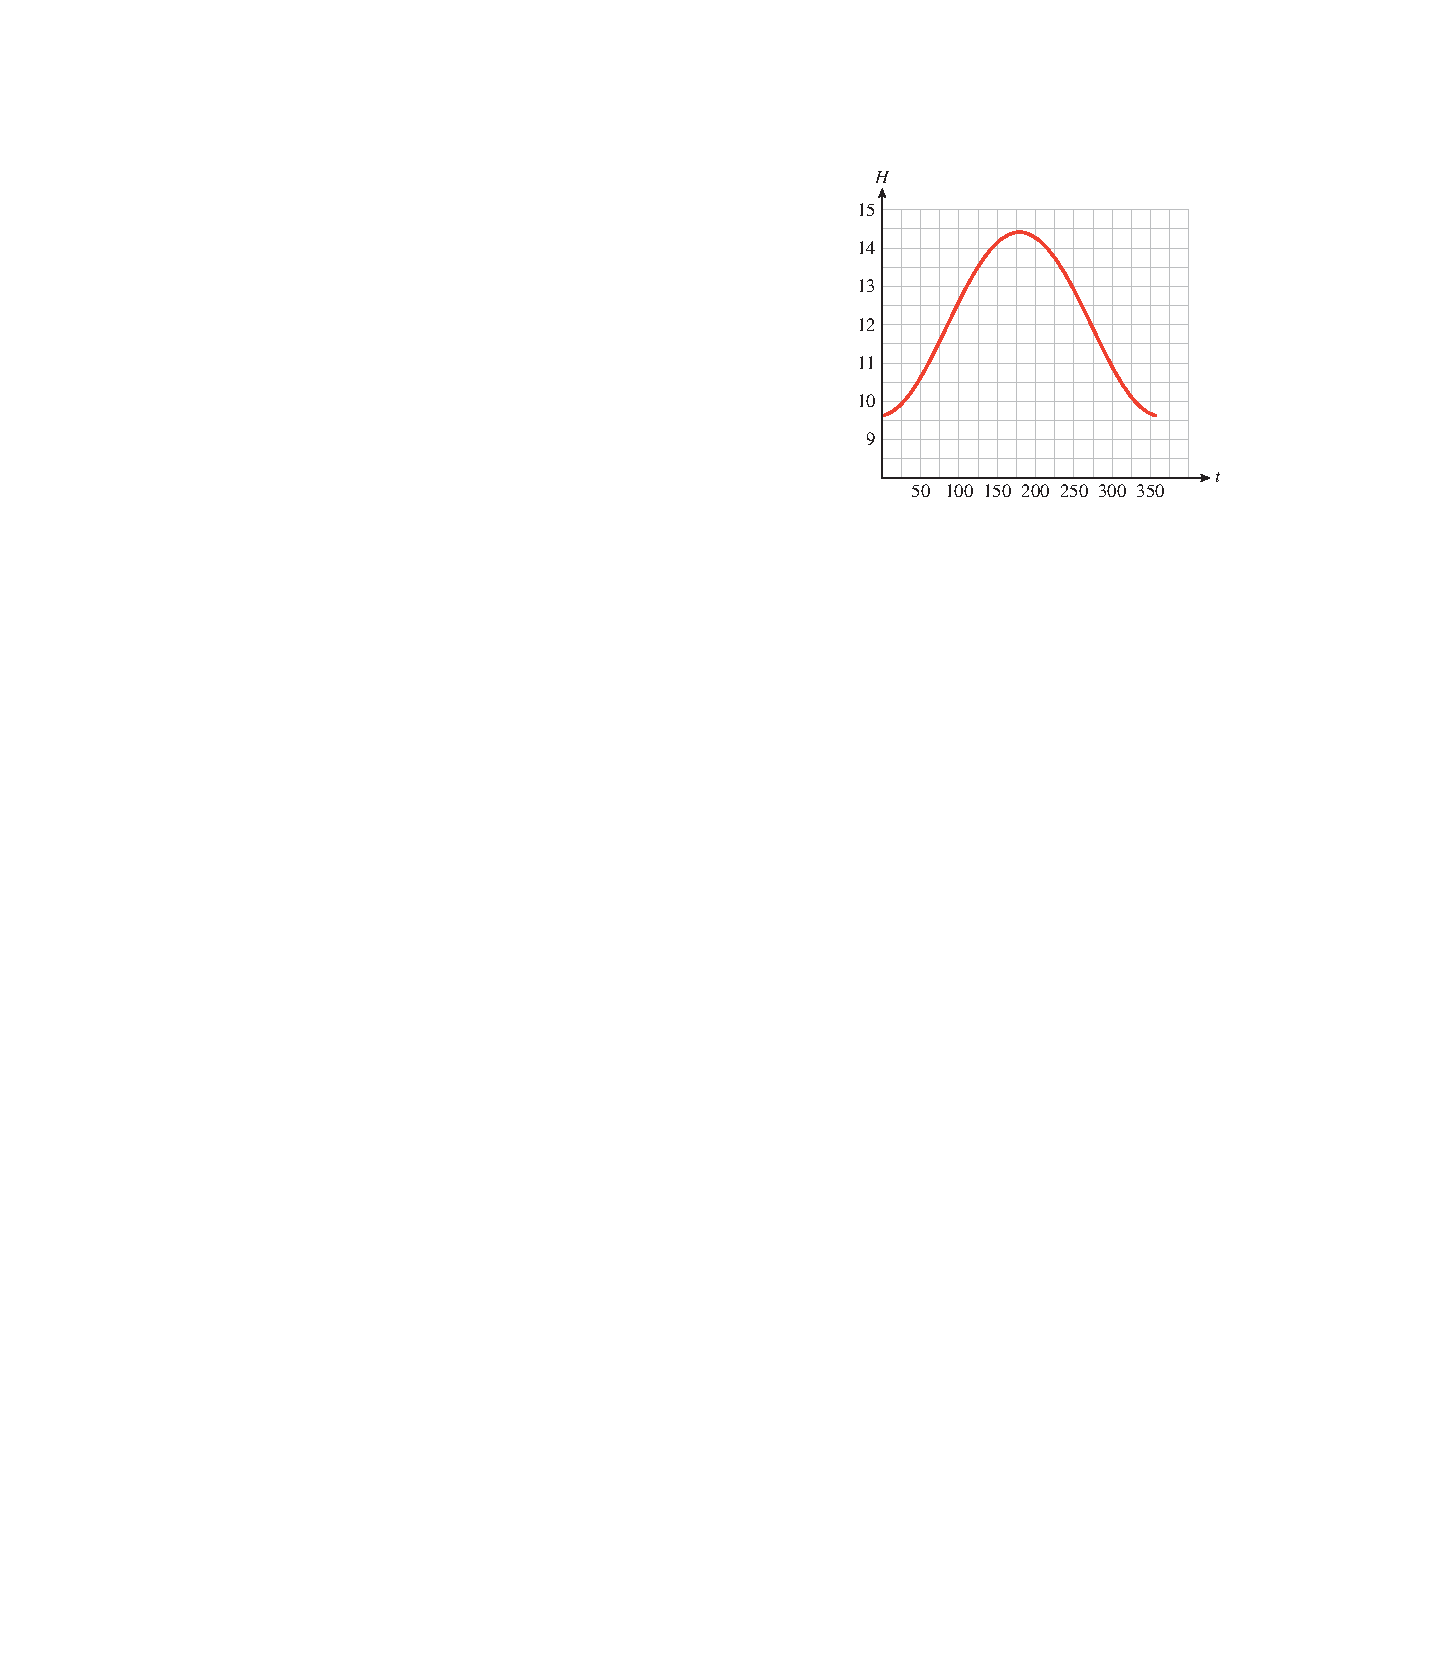
\includegraphics[width=0.4\linewidth]{https://mathbooks.unl.edu/PreCalculus/images/fig-sun-hours.pdf}
\end{lrbox}
\ifdefined\phAimage\else\newlength{\phAimage}\fi%
\setlength{\phAimage}{\ht\panelboxAimage+\dp\panelboxAimage}
\settototalheight{\phAimage}{\usebox{\panelboxAimage}}
\setlength{\panelmax}{\maxof{\panelmax}{\phAimage}}
\leavevmode%
% begin: side-by-side as tabular
% \tabcolsep change local to group
\setlength{\tabcolsep}{0.025\linewidth}
% @{} suppress \tabcolsep at extremes, so margins behave as intended
\par\medskip\noindent
\hspace*{0.025\linewidth}%
\begin{tabular}{@{}*{2}{c}@{}}
\begin{minipage}[c][\panelmax][t]{0.5\linewidth}\usebox{\panelboxAp}\end{minipage}&
\begin{minipage}[c][\panelmax][t]{0.4\linewidth}\usebox{\panelboxAimage}\end{minipage}\tabularnewline
&
\parbox[t]{0.4\linewidth}{\captionof{figure}{\label{fig-sun-hours}}
}\end{tabular}\\
% end: side-by-side as tabular
}% end: group for a single side-by-side
\end{example}
\hypertarget{p-39}{}%
We have a method of quickly determining if a relationship is a function once we have a graph of the relationship.%
\begin{assemblage}[The Vertical Line Test]\label{assemblage-2}
\hypertarget{p-40}{}%
A graph represents a function if and only if every vertical line intersects the graph in at most one point.%
\end{assemblage}
\begin{figure}
\centering
\centerline{Geogebra: \href{https://www.geogebra.org/m/j9j59n7z}{\mono{www.geogebra.org/m/j9j59n7z}}}
\caption{Demonstration of the Vertical Line Test\label{figure-2}}
\end{figure}
\begin{example}[]\label{example-vertical-line-test}
\hypertarget{p-41}{}%
Use the vertical line test to decide which of the graphs in \hyperref[fig-vertical-line-test2]{Figure~\ref{fig-vertical-line-test2}}  represent functions.%
\begin{figure}
\centering
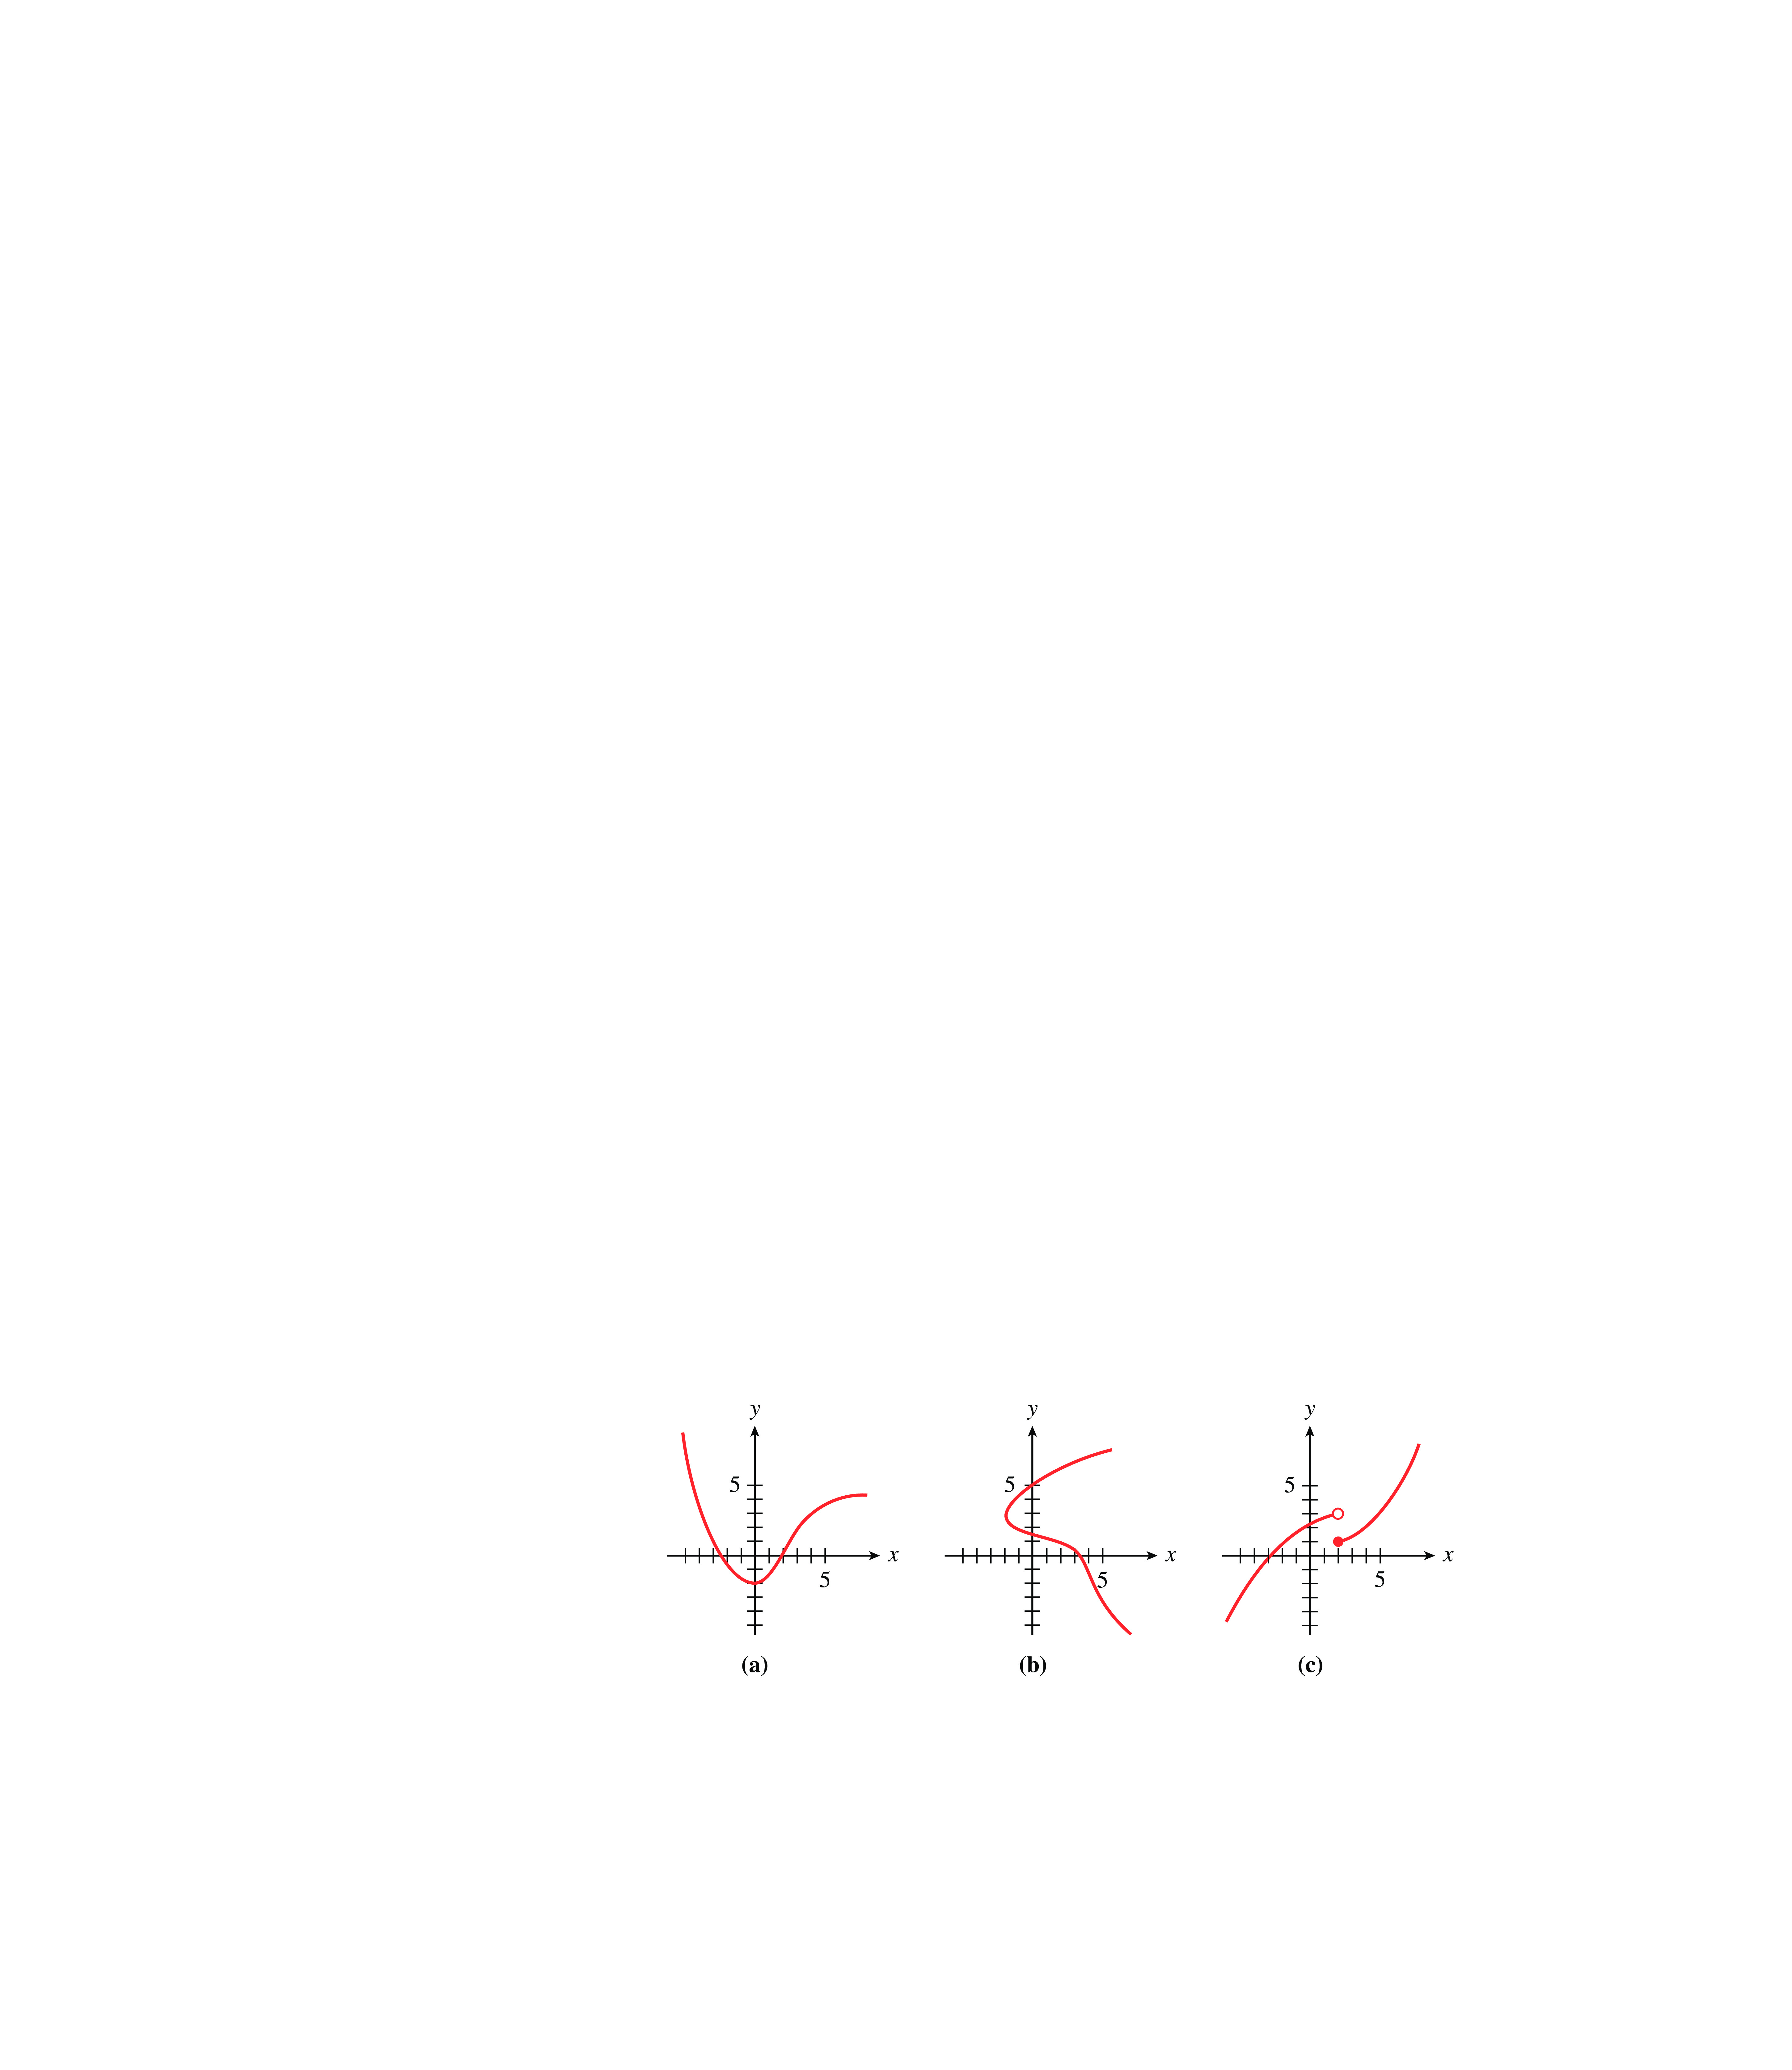
\includegraphics[width=0.9\linewidth]{images/fig-vertical-line-test2}
\caption{\label{fig-vertical-line-test2}}
\end{figure}
\par\smallskip%
\noindent\textbf{Solution.}\hypertarget{solution-1}{}\quad%
\hypertarget{p-42}{}%
\leavevmode%
\begin{itemize}[label=\textbullet]
\item{}\hypertarget{p-43}{}%
Graph (a) represents a function, because it passes the vertical line test.%
\item{}\hypertarget{p-44}{}%
Graph (b) is not the graph of a function, because the vertical line at (for example) \(x = 1\) intersects the graph at two points.%
\item{}\hypertarget{p-45}{}%
For graph (c), notice the break in the curve at \(x = 2\): The solid dot at \((2, 1)\) is the only point on the graph with \(x = 2\); the open circle at \((2, 3)\) indicates that \((2, 3)\) is not a point on the graph. Thus, graph (c) is a function, with \(f(2) = 1\).%
\end{itemize}
%
\end{example}
\typeout{************************************************}
\typeout{Subsection 1.4 Functions Defined by Equations}
\typeout{************************************************}
\section[{Functions Defined by Equations}]{Functions Defined by Equations}\label{subsection-4}
\hypertarget{p-46}{}%
\hyperref[example-falling-book]{Example~\ref{example-falling-book}} illustrates a function defined by an equation.%
\begin{example}[]\label{example-falling-book}
\hypertarget{p-47}{}%
As of 2016,  One World Trade Center in New York City is the nations tallest building, at 1776 feet. If an algebra book is dropped from the top of One World Trade Center, its height above the ground after \(t\) seconds is given by the equation%
\begin{equation*}
h = 1776 - 16t^2
\end{equation*}
Thus, after \(1\) second the books height is%
\begin{equation*}
h = 1776 - 16(1)^2 = 1760 \text{ feet}
\end{equation*}
After \(2\) seconds its height is%
\begin{equation*}
h = 1776 - 16(2)^2 = 1712 \text{ feet}
\end{equation*}
For this function, \(t\) is the input variable and \(h\) is the output variable. For any value of \(t\), a unique value of \(h\) can be determined from the equation for \(h\). We say that \(h\) \emph{is a function of} \(t\).%
\end{example}
\typeout{************************************************}
\typeout{Subsection 1.5 Function Notation}
\typeout{************************************************}
\section[{Function Notation}]{Function Notation}\label{subsection-5}
\hypertarget{p-48}{}%
There is a convenient notation for discussing functions. First, we choose a letter, such as \(f\), \(g\), or \(h\) (or \(F\), \(G\), or \(H\)), to name a particular function. (We can use any letter, but these are the most common choices.) For instance, the height, \(h\), of a falling textbook is a function of the elapsed time, \(t\). We might call this function \(f\). In other words, \(f\) is the name of the relationship between the variables \(h\) and \(t\). We write%
\begin{equation*}
h = f (t)
\end{equation*}
which means "\(h\) is a function of \(t\), and \(f\) is the name of the function."%
\begin{example}[]\label{example-falling-book-2}
\hypertarget{p-49}{}%
In \hyperref[example-falling-book]{Example~\ref{example-falling-book}}, the height of an algebra book dropped from the top of One World Trade Center is given by the equation%
\begin{equation*}
h = 1776 - 16t^2
\end{equation*}
We see that%
\par
\hypertarget{p-50}{}%
% group protects changes to lengths, releases boxes (?)
{% begin: group for a single side-by-side
% set panel max height to practical minimum, created in preamble
\setlength{\panelmax}{0pt}
\ifdefined\panelboxAtabular\else\newsavebox{\panelboxAtabular}\fi%
\savebox{\panelboxAtabular}{%
\raisebox{\depth}{\parbox{1\linewidth}{\centering\begin{tabular}{lll}
when \(t=1\)&&\(h=1760\)\tabularnewline[0pt]
when \(t=2\)&&\(h=1712\)
\end{tabular}
}}}
\ifdefined\phAtabular\else\newlength{\phAtabular}\fi%
\setlength{\phAtabular}{\ht\panelboxAtabular+\dp\panelboxAtabular}
\settototalheight{\phAtabular}{\usebox{\panelboxAtabular}}
\setlength{\panelmax}{\maxof{\panelmax}{\phAtabular}}
\leavevmode%
% begin: side-by-side as tabular
% \tabcolsep change local to group
\setlength{\tabcolsep}{0\linewidth}
% @{} suppress \tabcolsep at extremes, so margins behave as intended
\par\medskip\noindent
\begin{tabular}{@{}*{1}{c}@{}}
\begin{minipage}[c][\panelmax][t]{1\linewidth}\usebox{\panelboxAtabular}\end{minipage}\end{tabular}\\
% end: side-by-side as tabular
}% end: group for a single side-by-side
%
\par
\hypertarget{p-51}{}%
Using function notation, these relationships can be expressed more concisely as%
\par
\hypertarget{p-52}{}%
% group protects changes to lengths, releases boxes (?)
{% begin: group for a single side-by-side
% set panel max height to practical minimum, created in preamble
\setlength{\panelmax}{0pt}
\ifdefined\panelboxAtabular\else\newsavebox{\panelboxAtabular}\fi%
\savebox{\panelboxAtabular}{%
\raisebox{\depth}{\parbox{1\linewidth}{\centering\begin{tabular}{lll}
\(f(1)=1760\)&and&\(f(2)=1712\)
\end{tabular}
}}}
\ifdefined\phAtabular\else\newlength{\phAtabular}\fi%
\setlength{\phAtabular}{\ht\panelboxAtabular+\dp\panelboxAtabular}
\settototalheight{\phAtabular}{\usebox{\panelboxAtabular}}
\setlength{\panelmax}{\maxof{\panelmax}{\phAtabular}}
\leavevmode%
% begin: side-by-side as tabular
% \tabcolsep change local to group
\setlength{\tabcolsep}{0\linewidth}
% @{} suppress \tabcolsep at extremes, so margins behave as intended
\par\medskip\noindent
\begin{tabular}{@{}*{1}{c}@{}}
\begin{minipage}[c][\panelmax][t]{1\linewidth}\usebox{\panelboxAtabular}\end{minipage}\end{tabular}\\
% end: side-by-side as tabular
}% end: group for a single side-by-side
%
\par
\hypertarget{p-53}{}%
which we read as "\(f\) of 1 equals 1760" and "\(f\) of 2 equals 1712." The values for the input variable, \(t\), appear \emph{inside} the parentheses, and the values for the output variable, \(h\), appear on the other side of the equation.%
\end{example}
\hypertarget{p-54}{}%
Remember that when we write \(y = f(x)\), the symbol \(f(x)\) is just another name for the output variable.%
\typeout{************************************************}
\typeout{Subsection 1.6 Evaluating a Function}
\typeout{************************************************}
\section[{Evaluating a Function}]{Evaluating a Function}\label{subsection-6}
\hypertarget{p-55}{}%
Finding the value of the output variable that corresponds to a particular value of the input variable is called \terminology{evaluating the function}\index{evaluating the function}.%
\begin{example}[]\label{example-postage2}
\hypertarget{p-56}{}%
Let \(g\) be the name of the postage function defined by \hyperref[table-postage]{Table~\ref{table-postage}}. Find \(g(1)\), \(g(3)\), and \(g(6.75\)).%
\par\smallskip%
\noindent\textbf{Solution.}\hypertarget{solution-2}{}\quad%
\hypertarget{p-57}{}%
According to the table,%
\par
\hypertarget{p-58}{}%
% group protects changes to lengths, releases boxes (?)
{% begin: group for a single side-by-side
% set panel max height to practical minimum, created in preamble
\setlength{\panelmax}{0pt}
\ifdefined\panelboxAtabular\else\newsavebox{\panelboxAtabular}\fi%
\savebox{\panelboxAtabular}{%
\raisebox{\depth}{\parbox{1\linewidth}{\centering\begin{tabular}{lllll}
when \(w=1\),&&\(p=0.47\)&so&\(g(1)=0.47\)\tabularnewline[0pt]
when \(w=3\),&&\(p=0.89\)&so&\(g(3)=0.89\)\tabularnewline[0pt]
when \(w=6.75\),&&\(p=1.73\)&so&\(g(6.75)=1.73\)
\end{tabular}
}}}
\ifdefined\phAtabular\else\newlength{\phAtabular}\fi%
\setlength{\phAtabular}{\ht\panelboxAtabular+\dp\panelboxAtabular}
\settototalheight{\phAtabular}{\usebox{\panelboxAtabular}}
\setlength{\panelmax}{\maxof{\panelmax}{\phAtabular}}
\leavevmode%
% begin: side-by-side as tabular
% \tabcolsep change local to group
\setlength{\tabcolsep}{0\linewidth}
% @{} suppress \tabcolsep at extremes, so margins behave as intended
\par\medskip\noindent
\begin{tabular}{@{}*{1}{c}@{}}
\begin{minipage}[c][\panelmax][t]{1\linewidth}\usebox{\panelboxAtabular}\end{minipage}\end{tabular}\\
% end: side-by-side as tabular
}% end: group for a single side-by-side
 Thus, a letter weighing 1 ounce costs \textdollar{}0.47 to mail, a letter weighing 3 ounces costs \textdollar{}0.89, and a letter weighing 6.75 ounces costs \textdollar{}1.73.%
\end{example}
\hypertarget{p-59}{}%
If a function is described by an equation, we simply substitute the given input value into the equation to find the corresponding output, or function value.%
\begin{example}[]\label{example-evaluate-function}
\hypertarget{p-60}{}%
The function \(H\) is defined by \(H=f(s) = \dfrac{\sqrt{s+3}}{s}\). Evaluate the function at the following values. \leavevmode%
\begin{enumerate}[label=\alph*]
\item\hypertarget{li-14}{}\hypertarget{p-61}{}%
\(s=6\)%
\item\hypertarget{li-15}{}\hypertarget{p-62}{}%
\(s=-1\)%
\end{enumerate}
%
\par\smallskip%
\noindent\textbf{Solution.}\hypertarget{solution-3}{}\quad%
\hypertarget{p-63}{}%
\leavevmode%
\begin{enumerate}[label=\alph*]
\item\hypertarget{li-16}{}\hypertarget{p-64}{}%
\(f(\alert{6})=\dfrac{\sqrt{\alert{6}+3}}{\alert{6}}=
\dfrac{\sqrt{9}}{6}=\dfrac{3}{6}=\dfrac{1}{2}\). Thus, \(f(6)=\dfrac{1}{2}\).%
\item\hypertarget{li-17}{}\hypertarget{p-65}{}%
\(f(\alert{-1})=\dfrac{\sqrt{\alert{-1}+3}}{\alert{-1}}=
\dfrac{\sqrt{2}}{-1}=-\sqrt{2}\). Thus, \(f(-1)=-\sqrt{2}\).%
\end{enumerate}
%
\end{example}
\hypertarget{p-66}{}%
To simplify the notation, we sometimes use the same letter for the output variable and for the name of the function.%
\typeout{************************************************}
\typeout{Subsection 1.7 Linear Functions}
\typeout{************************************************}
\section[{Linear Functions}]{Linear Functions}\label{subsection-7}
\hypertarget{p-67}{}%
Linear relationships are relationships in which the rate of change is constant. \begin{assemblage}[Linear Equation]\label{assemblage-3}
\hypertarget{p-68}{}%
A \terminology{linear function} is a function which has a \terminology{constant rate of change.}%
\end{assemblage}
 Many phenomena can be modeled using linear functions \(y = f (x)\) where the equations have the form%
\begin{equation*}
f (x) = (\text{starting value}) + (\text{rate of change}) \cdot x.
\end{equation*}
The initial value, or the value of \(f(0)\), is the vertical intercept of the graph, and the rate of change is the slope of the graph. Thus, we can write an equation of a line as%
\begin{equation*}
f (x) = b + mx
\end{equation*}
where the constant term, \(b\), is the vertical intercept of the line, and \(m\), the coefficient of \(x\), is the slope of the line. This form for an equation of a line is called the \terminology{slope-intercept form}\index{slope-intercept form}.%
\begin{assemblage}[Slope-Intercept Form]\label{assemblage-4}
\hypertarget{p-69}{}%
If we write an equation of a linear function in the form,%
\begin{equation*}
f (x) = b + mx
\end{equation*}
then \(m\) is the \terminology{slope}\index{slope} of the line, and \(b\) is the \terminology{vertical intercept}.%
\end{assemblage}
\begin{example}[]\label{example-linear-function1}
\hypertarget{p-70}{}%
An icicle grows according to the formula \(H(t)=0.05t+0.12\), where \(t\) is the time in minutes since the first measurement was take, and \(H(t)\) is the height of the icicle in centimeters.%
\par
\hypertarget{p-71}{}%
\leavevmode%
\begin{enumerate}[label=\alph*]
\item\hypertarget{li-18}{}\hypertarget{p-72}{}%
The slope is 0.05, which tells us that the icicle's height grows by 0.05 cm each minute.%
\item\hypertarget{li-19}{}\hypertarget{p-73}{}%
The \(y\)-intercept is 0.12, which tells us that the height of the icicle was 0.12 cm at the first measurement.%
\end{enumerate}
%
\end{example}
\begin{example}[]\label{example-linear-function2}
\hypertarget{p-74}{}%
Samantha owns a catering business. For any party with up to 100 guests, she charges $2,000. She charges $8 per person for each additional guest over 100. Give a formula for the cost of having Samantha cater your party as a function of the number of guests over 200.%
\par\smallskip%
\noindent\textbf{Solution.}\hypertarget{solution-4}{}\quad%
\hypertarget{p-75}{}%
A possible formula for the cost of having Samantha cater your party is \(C(g)=2000+8g\), where \(g\) is the number of guests over 100.%
\end{example}
\hypertarget{p-76}{}%
The following formula provides a method to finding the value of the slope \(m\) when given two points on the line.%
\begin{assemblage}[Two-Point Slope Formula]\label{assemblage-5}
\hypertarget{p-77}{}%
The slope of the line passing through the points \(P_1 (x_1, y_1)\) and \(P_2 (x_2, y_2)\) is given by%
\begin{equation*}
m = \frac{\Delta y}{\Delta x}= \frac{y_2 - y_1}{x_2 - x_1} 
\text{, }~x_2 \ne x_1.
\end{equation*}
%
\end{assemblage}
\begin{example}[]\label{example-two-point-slope}
\hypertarget{p-78}{}%
Compute the slope of the line between the points \((6, -3)\) and \((4, 3)\).%
\par\smallskip%
\noindent\textbf{Solution.}\hypertarget{solution-5}{}\quad%
\hypertarget{p-79}{}%
Substitute the coordinates of \(Q_1\) and \(Q_2\) into the slope formula to find%
\begin{equation*}
m = \frac{y_2 - y_1}{x_2 - x_1}= \frac{3 - (-3)}{4 - 6}
= \frac{6}{-2}= -3.
\end{equation*}
This value for the slope, \(-3\), is the same value found above.%
\end{example}
\hypertarget{p-80}{}%
Sometimes you will be given the slope of a line and another point on that line. The following formula is helpful in that situation.%
\begin{assemblage}[Point-Slope Form]\label{assemblage-6}
\hypertarget{p-81}{}%
An equation of the line that passes through the point \((x_1, y_1)\) and has slope \(m\) is%
\begin{equation*}
y= y_1 + m(x- x_1).
\end{equation*}
%
\end{assemblage}
\begin{example}[]\label{example-point-slope2}
\hypertarget{p-82}{}%
Find a formula for the line that has slope -2 and passes through the point \((-1,4)\)%
\par\smallskip%
\noindent\textbf{Solution.}\hypertarget{solution-6}{}\quad%
\hypertarget{p-83}{}%
Using point-slope form, we have the line \(y=4+(-2)(x-(-1))\).%
\par
\hypertarget{p-84}{}%
We can also write this in slope-intercept form by simplifying: \(y=2-2x\).%
\end{example}
\hypertarget{p-85}{}%
Is is also useful to introduce the term \(x\)-intercept. \begin{assemblage}[\(x\)-intercept]\label{assemblage-7}
\hypertarget{p-86}{}%
An \terminology{\(x\)-intercept} for a function \(f(x)\) is the value of \(x\) such that \(f(x)=0\).%
\end{assemblage}
%
\begin{note}[]\label{note-1}
\hypertarget{p-87}{}%
In the equation \(f (x) = b + mx\), we call \(m\) and \(b\) \terminology{parameters}\index{parameters}. Their values are fixed for any particular linear equation; for example, in the equation \(y = 2x + 3\), \(m = 2\) and \(b = 3\), and the variables are \(x\) and \(y\). By changing the values of \(m\) and \(b\), we can write the equation for any line except a vertical line (see \hyperref[fig-slope-vs-intercept]{Figure~\ref{fig-slope-vs-intercept}}). The collection of all linear functions \(f (x) = b + mx\) is called a \terminology{two-parameter}\index{two-parameter} family of functions.%
\end{note}
\begin{figure}
\centering
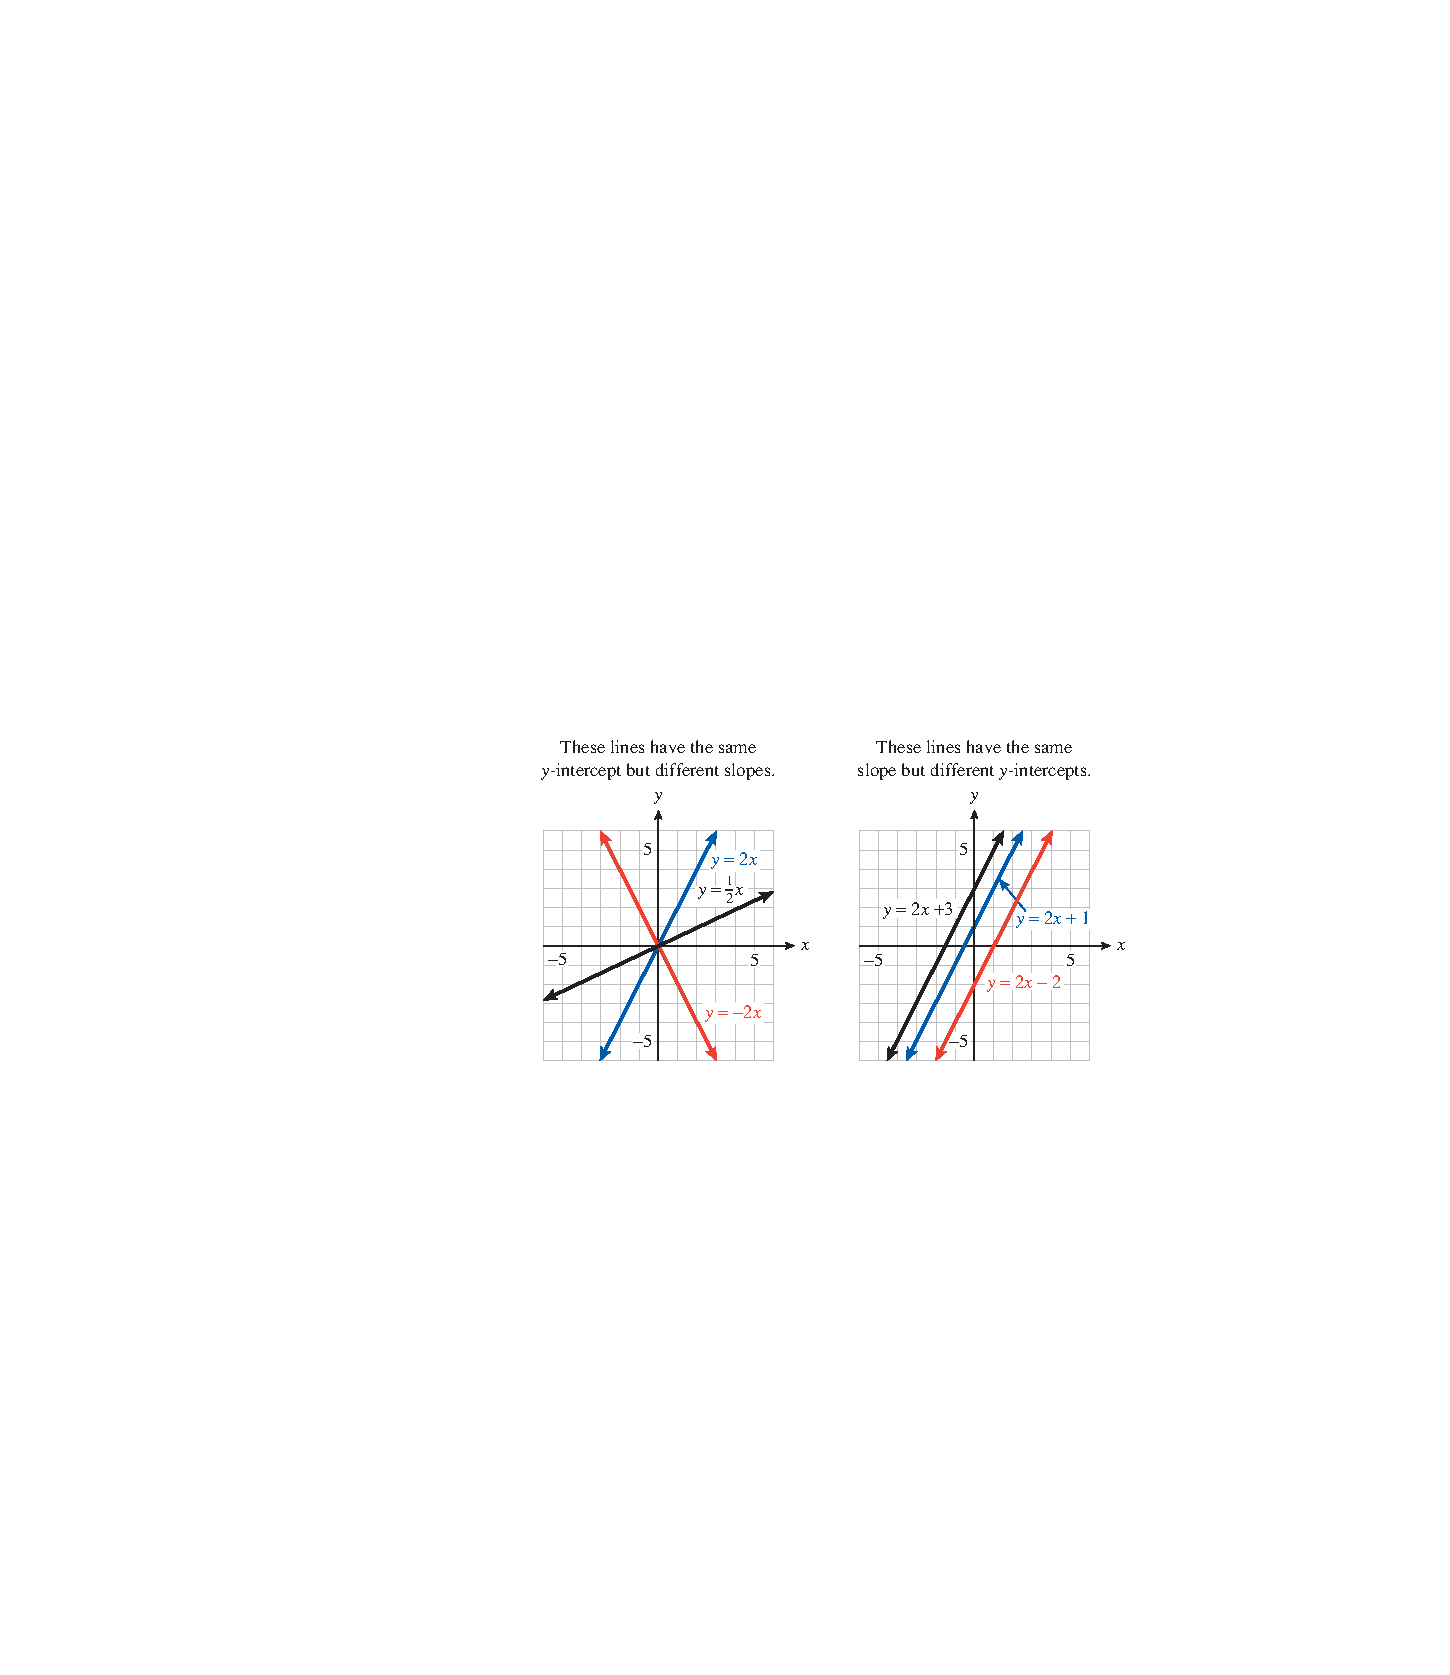
\includegraphics[width=0.8\linewidth]{https://mathbooks.unl.edu/PreCalculus/images/fig-slope-vs-intercept.pdf}
\caption{\label{fig-slope-vs-intercept}}
\end{figure}
\typeout{************************************************}
\typeout{Subsection 1.8 Describing Functions}
\typeout{************************************************}
\section[{Describing Functions}]{Describing Functions}\label{subsection-8}
\hypertarget{p-88}{}%
There are several terms that will be useful in describing functions.  We first begin with the notion of an increasing function.%
\begin{assemblage}[Increasing Function]\label{assemblage-8}
\hypertarget{p-89}{}%
A function \(f\) is increasing if the values of \(f(x)\) increase as \(x\) increases. The graph of an increasing function climbs as we move from left to right.%
\end{assemblage}
\begin{assemblage}[Decreasing Function]\label{assemblage-9}
\hypertarget{p-90}{}%
A function \(f\) is decreasing if the values of \(f(x)\) decrease as \(x\) increases. The graph of a decreasing function falls as we move from left to right.%
\end{assemblage}
\begin{assemblage}[Monotonic Funcion]\label{assemblage-10}
\hypertarget{p-91}{}%
A function \(f(x)\) is monotonic if it increases for all \(x\) or decreases for all \(x\).%
\end{assemblage}
\begin{assemblage}[Directly Proportional]\label{assemblage-11}
\hypertarget{p-92}{}%
We say \(y\) is directly proportional to \(x\) if there is a nonzero constant \(k\) such that, \(y = kx\). This \(k\) is called the constant of proportionality.%
\end{assemblage}
\begin{assemblage}[Inversely Proportional]\label{assemblage-12}
\hypertarget{p-93}{}%
We say that \(y\) is inversely proportional to \(x\) if \(y\) is proportional to the reciprocal of \(x\), that is, \(y = \frac{k}{x}\) for a nonzero constant \(k\).%
\end{assemblage}
\typeout{************************************************}
\typeout{Subsection 1.9 Function Transformations}
\typeout{************************************************}
\section[{Function Transformations}]{Function Transformations}\label{subsection-9}
\hypertarget{p-94}{}%
It is also useful to talk about transformations of functions.  Several key facts will be useful.%
\begin{assemblage}[Function Transformations]\label{assemblage-13}
\hypertarget{p-95}{}%
\leavevmode%
\begin{enumerate}
\item\hypertarget{li-20}{}Multiplying a function by a constant, \(c\), stretches the graph vertically (if \(c \gt 1\)) or shrinks the graph vertically (if \(0 \lt c \lt 1\))%
\item\hypertarget{li-21}{}A negative sign (if \(c \lt 0\)) reflects the graph about the \(x\)-axis, in addition to shrinking or stretching.%
\item\hypertarget{li-22}{}Replacing \(y\) by \((y+k)\) moves a graph up by \(k\) (down if \(k\) is negative).%
\item\hypertarget{li-23}{}Replacing \(x\) by \((x-h)\) moves a graph to the right by \(h\) (to the left if \(h\) is negative).%
\end{enumerate}
%
\end{assemblage}
\begin{example}[]\label{example-12}
\hypertarget{p-96}{}%
Let \(f(x)=x^2\). We will explore different transformations performed on the graph of \(f(x)\).%
\par
\hypertarget{p-97}{}%
\leavevmode%
\begin{enumerate}[label=\alph*]
\item\hypertarget{li-24}{}\hypertarget{p-98}{}%
\(g(x)=2\cdotf(x)=2x^2\) is a vertical stretch of \(f(x)\) by a factor of 2.%
\item\hypertarget{li-25}{}\hypertarget{p-99}{}%
\(h(x)=-2\cdotf(x)=-2x^2\) is a vertical stretch of \(f(x)\) by a factor of 2 and a reflection across the \(x\)-axis.%
\item\hypertarget{li-26}{}\hypertarget{p-100}{}%
\(j(x)=f(x)+5=x^2+5\) is a vertical shift of \(f(x)\) up 5 units.%
\item\hypertarget{li-27}{}\hypertarget{p-101}{}%
\(k(x)=f(x+5)=(x+5)^2\) is a horizontal shift of \(f(x)\) left 5 units.%
\end{enumerate}
%
\end{example}
\begin{assemblage}[Order of Transformations]\label{assemblage-14}
\hypertarget{p-102}{}%
Suppose that \(f(x)\) is our function we are applying transformations to. Once written in the form%
\begin{equation*}
a\cdot f(b\cdot (x+h))+k
\end{equation*}
the order of transformations is:%
\par
\hypertarget{p-103}{}%
\leavevmode%
\begin{enumerate}
\item\hypertarget{li-28}{}horizontal stretch or compress by a factor of \(\abs{b}\) or \(\abs{\dfrac{1}{b}}\) (if \(b\lt 0\) then also reflect about \(y\)-axis)%
\item\hypertarget{li-29}{}shift horizontally left/ right by \(\abs{h} \)%
\item\hypertarget{li-30}{}vertically stretch or compress by a factor of \(\abs{a}\) or \(\abs{\dfrac{1}{a}}\) (if \(a\lt 0\) then also reflect about \(x\)-axis)%
\item\hypertarget{li-31}{}shift vertically up/ down by \(\abs{k} \)%
\end{enumerate}
%
\end{assemblage}
\begin{example}[]\label{example-13}
\hypertarget{p-104}{}%
Describe the function%
\begin{equation*}
5\cdot [f(-3x-6)-1]
\end{equation*}
as a list of transformations done to \(f(x)\) in the appropriate order.%
\par\smallskip%
\noindent\textbf{Solution.}\hypertarget{solution-7}{}\quad%
\hypertarget{p-105}{}%
First, let's rewrite the function in the form given above: \begin{align*} 5\cdot [f(-3x-6)-1]\amp = 5f(-3x-6)-5 \ \ \text{we distributed in the 5}\\ \amp = 5f(-3(x+2))-5 \ \ \text{we factored out the -3} \end{align*} Now that the function is written in the desired order, we may list off the transformations in the correct order using the order discussed above: \leavevmode%
\begin{enumerate}
\item\hypertarget{li-32}{}horizontal compress by \(3\) and reflect about the \(y\)-axis%
\item\hypertarget{li-33}{}shift horizontally left by \(2 \)%
\item\hypertarget{li-34}{}vertically stretch by \(5\)%
\item\hypertarget{li-35}{}shift vertically down by \(5 \)%
\end{enumerate}
%
\end{example}
\typeout{************************************************}
\typeout{Subsection 1.10 Inverse Functions}
\typeout{************************************************}
\section[{Inverse Functions}]{Inverse Functions}\label{subsection-10}
\hypertarget{p-106}{}%
It is also useful to consider inverse functions.%
\begin{assemblage}[Inverse Functions]\label{assemblage-15}
\hypertarget{p-107}{}%
Suppose the inverse of \(f\) is a function, denoted by \(f^{-1}\). Then%
\begin{equation*}
f^{-1}(y) = x \text{ if and only if }f(x) = y.
\end{equation*}
%
\end{assemblage}
\begin{example}[]\label{example-inverse-functions}
\hypertarget{p-108}{}%
Suppose \(g\) is the inverse function for \(f\), and we know the following function values for \(f\):%
\begin{equation*}
f (-3) = 5, ~~ f (2) = 1, ~~ f (5) = 0.
\end{equation*}
Find \(g(5)\) and \(g(0)\).%
\par\smallskip%
\noindent\textbf{Solution.}\hypertarget{solution-8}{}\quad%
\hypertarget{p-109}{}%
We know that \(g(5) = -3\) because \(f (-3) = 5\), and \(g(0) = 5\) because \(f (5) = 0\). Tables may be helpful in visualizing the two functions, as shown below.%
% group protects changes to lengths, releases boxes (?)
{% begin: group for a single side-by-side
% set panel max height to practical minimum, created in preamble
\setlength{\panelmax}{0pt}
\ifdefined\panelboxAtabular\else\newsavebox{\panelboxAtabular}\fi%
\savebox{\panelboxAtabular}{%
\raisebox{\depth}{\parbox{0.19\linewidth}{\centering\begin{tabular}{AcAcA}\hrulethick
\multicolumn{2}{AcA}{\(y=f(x)\)}\tabularnewline\hrulethin
\(x\)&\(y\)\tabularnewline\hrulethin
\(-3\)&\(5\)\tabularnewline\hrulethin
\(2\)&\(1\)\tabularnewline\hrulethin
\(5\)&\(0\)\tabularnewline\hrulethin
\end{tabular}
}}}
\ifdefined\phAtabular\else\newlength{\phAtabular}\fi%
\setlength{\phAtabular}{\ht\panelboxAtabular+\dp\panelboxAtabular}
\settototalheight{\phAtabular}{\usebox{\panelboxAtabular}}
\setlength{\panelmax}{\maxof{\panelmax}{\phAtabular}}
\ifdefined\panelboxAp\else\newsavebox{\panelboxAp}\fi%
\savebox{\panelboxAp}{%
\raisebox{\depth}{\parbox{0.45\linewidth}{→ Interchange the columns →}}}
\ifdefined\phAp\else\newlength{\phAp}\fi%
\setlength{\phAp}{\ht\panelboxAp+\dp\panelboxAp}
\settototalheight{\phAp}{\usebox{\panelboxAp}}
\setlength{\panelmax}{\maxof{\panelmax}{\phAp}}
\ifdefined\panelboxBtabular\else\newsavebox{\panelboxBtabular}\fi%
\savebox{\panelboxBtabular}{%
\raisebox{\depth}{\parbox{0.19\linewidth}{\centering\begin{tabular}{AcAcA}\hrulethick
\multicolumn{2}{AcA}{\(x=g(y)\)}\tabularnewline\hrulethin
\(y\)&\(x\)\tabularnewline\hrulethin
\(5\)&\(-3\)\tabularnewline\hrulethin
\(1\)&\(2\)\tabularnewline\hrulethin
\(0\)&\(5\)\tabularnewline\hrulethin
\end{tabular}
}}}
\ifdefined\phBtabular\else\newlength{\phBtabular}\fi%
\setlength{\phBtabular}{\ht\panelboxBtabular+\dp\panelboxBtabular}
\settototalheight{\phBtabular}{\usebox{\panelboxBtabular}}
\setlength{\panelmax}{\maxof{\panelmax}{\phBtabular}}
\leavevmode%
% begin: side-by-side as tabular
% \tabcolsep change local to group
\setlength{\tabcolsep}{0.0075\linewidth}
% @{} suppress \tabcolsep at extremes, so margins behave as intended
\par\medskip\noindent
\hspace*{0.07\linewidth}%
\begin{tabular}{@{}*{3}{c}@{}}
\begin{minipage}[c][\panelmax][c]{0.19\linewidth}\usebox{\panelboxAtabular}\end{minipage}&
\begin{minipage}[c][\panelmax][c]{0.45\linewidth}\usebox{\panelboxAp}\end{minipage}&
\begin{minipage}[c][\panelmax][c]{0.19\linewidth}\usebox{\panelboxBtabular}\end{minipage}\end{tabular}\\
% end: side-by-side as tabular
}% end: group for a single side-by-side
\par
\hypertarget{p-111}{}%
For the function \(f\), the input variable is \(x\) and the output variable is \(y\). For the inverse function \(g\), the roles of the variables are interchanged: \(y\) is now the input and \(x\) is the output.%
\end{example}
\begin{assemblage}[Functions and Inverse Functions]\label{assemblage-16}
\hypertarget{p-112}{}%
Suppose \(f^{-1}\) is the inverse function for \(f\). Then%
\begin{equation*}
f^{-1}\left(f(x)\right) = x\text{ and }f\left(f^{-1}( y)\right) = y
\end{equation*}
as long as \(x\) is in the domain of \(f\), and \(y\) is in the domain of \(f^{-1}\).%
\end{assemblage}
\hypertarget{p-113}{}%
We also have a method of quickly determining if a function is invertible once we have a graph of the function.%
\begin{assemblage}[Horizontal Line Test]\label{assemblage-17}
\hypertarget{p-114}{}%
If no horizontal line intersects the graph of a function more than once, then its inverse is also a function.%
\end{assemblage}
\begin{figure}
\centering
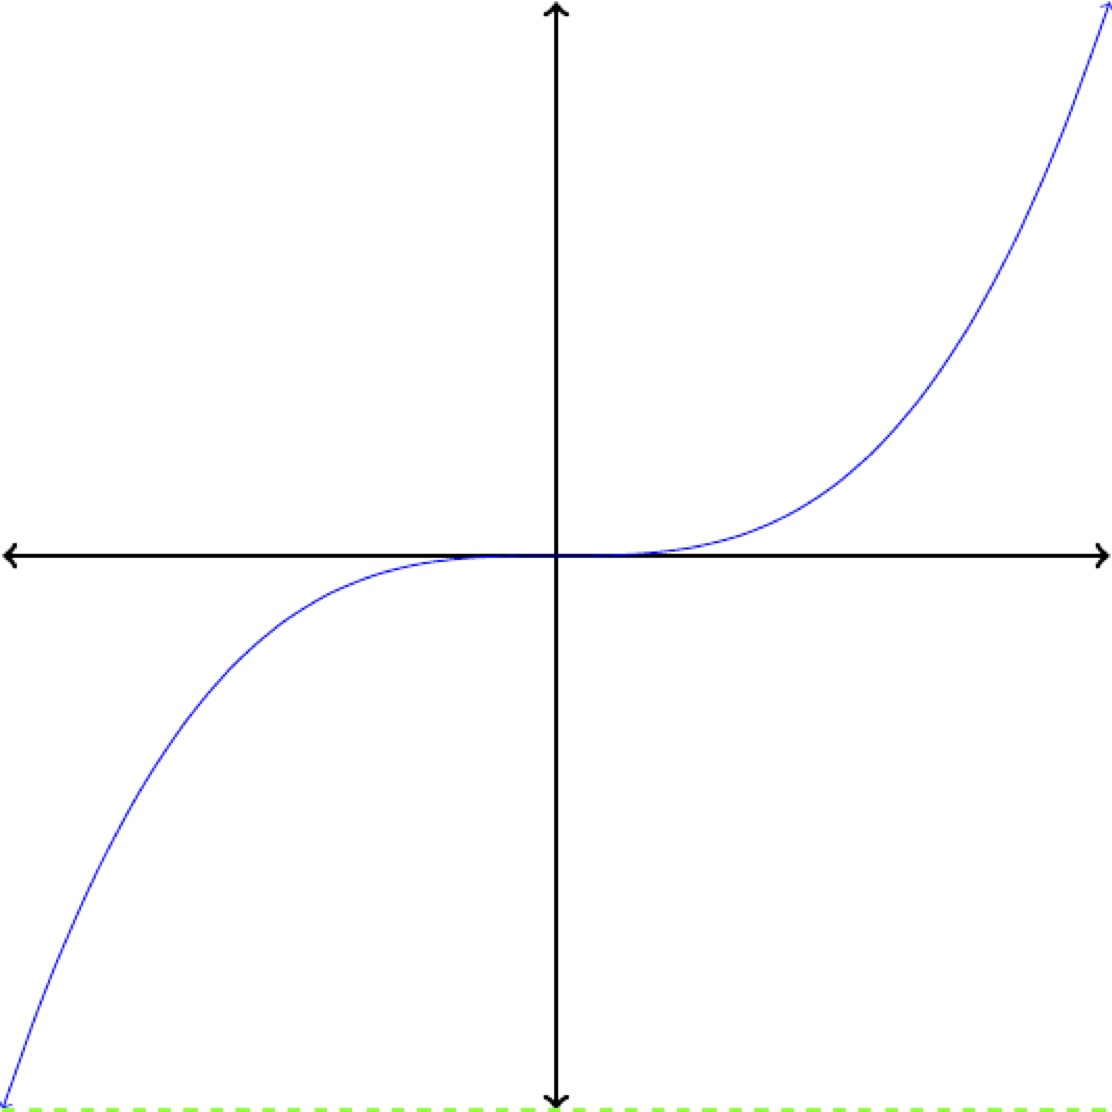
\includegraphics[width=0.7\linewidth]{images/HorizontalLineTest.gif}
\caption{Notice that as the line moves up the \(y-\) axis, it only ever intersects the graph in a single place.  This means this function is invertible.\label{fig-horizontal-line-test-animation}}
\end{figure}
\begin{figure}
\centering
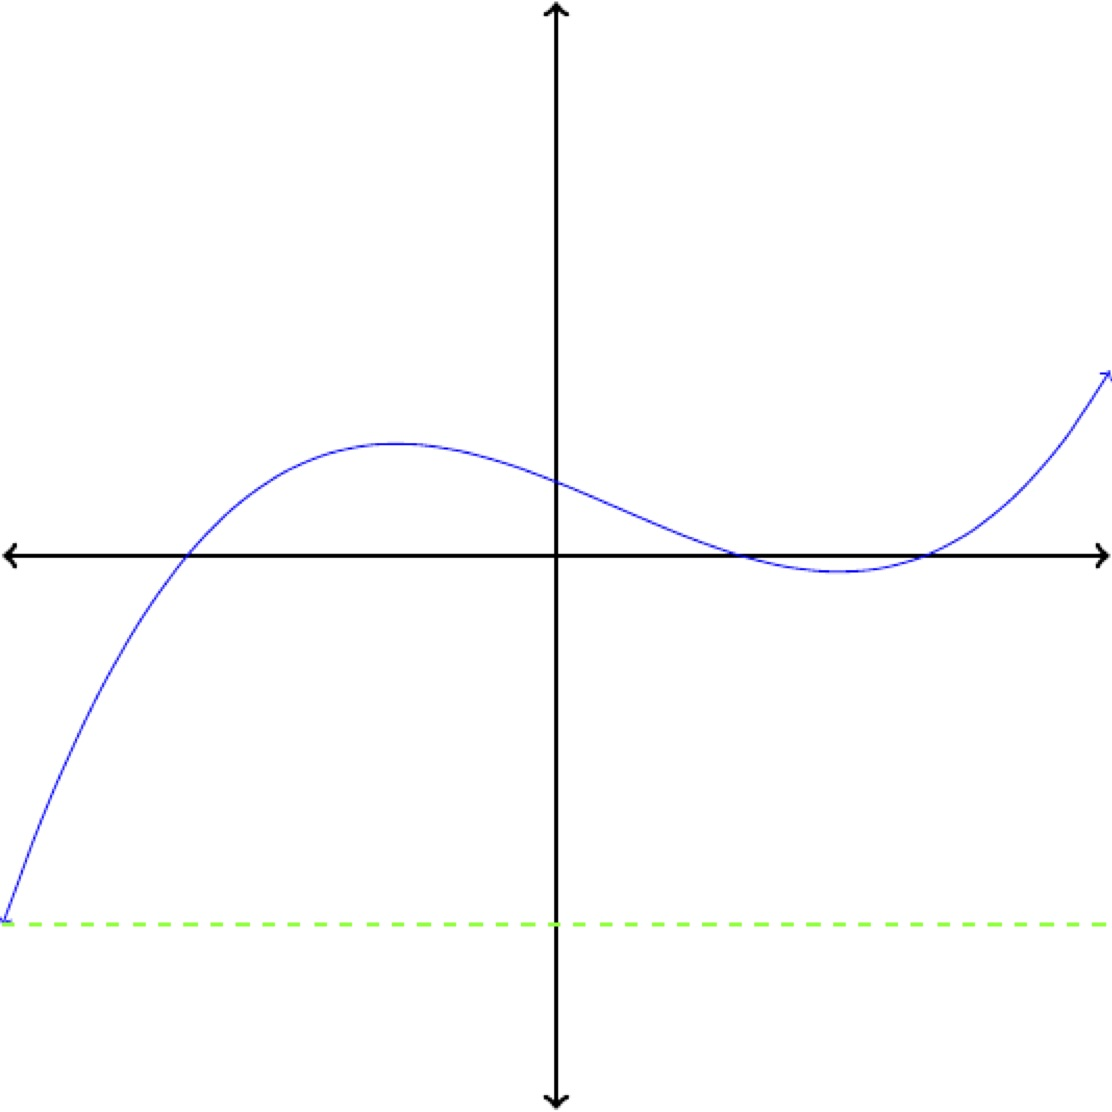
\includegraphics[width=0.7\linewidth]{images/HorizontalLineTestFail.gif}
\caption{Notice that as the line moves up the \(y-\) axis, it sometimes intersects the graph in more than one place.  This means this function is not invertible.\label{fig-horizontal-line-test-fail-animation}}
\end{figure}
\begin{example}[]\label{example-invertible-or-not}
\hypertarget{p-115}{}%
Which of the functions in \hyperref[fig-invertible-or-not]{Figure~\ref{fig-invertible-or-not}} are invertible?%
\begin{figure}
\centering
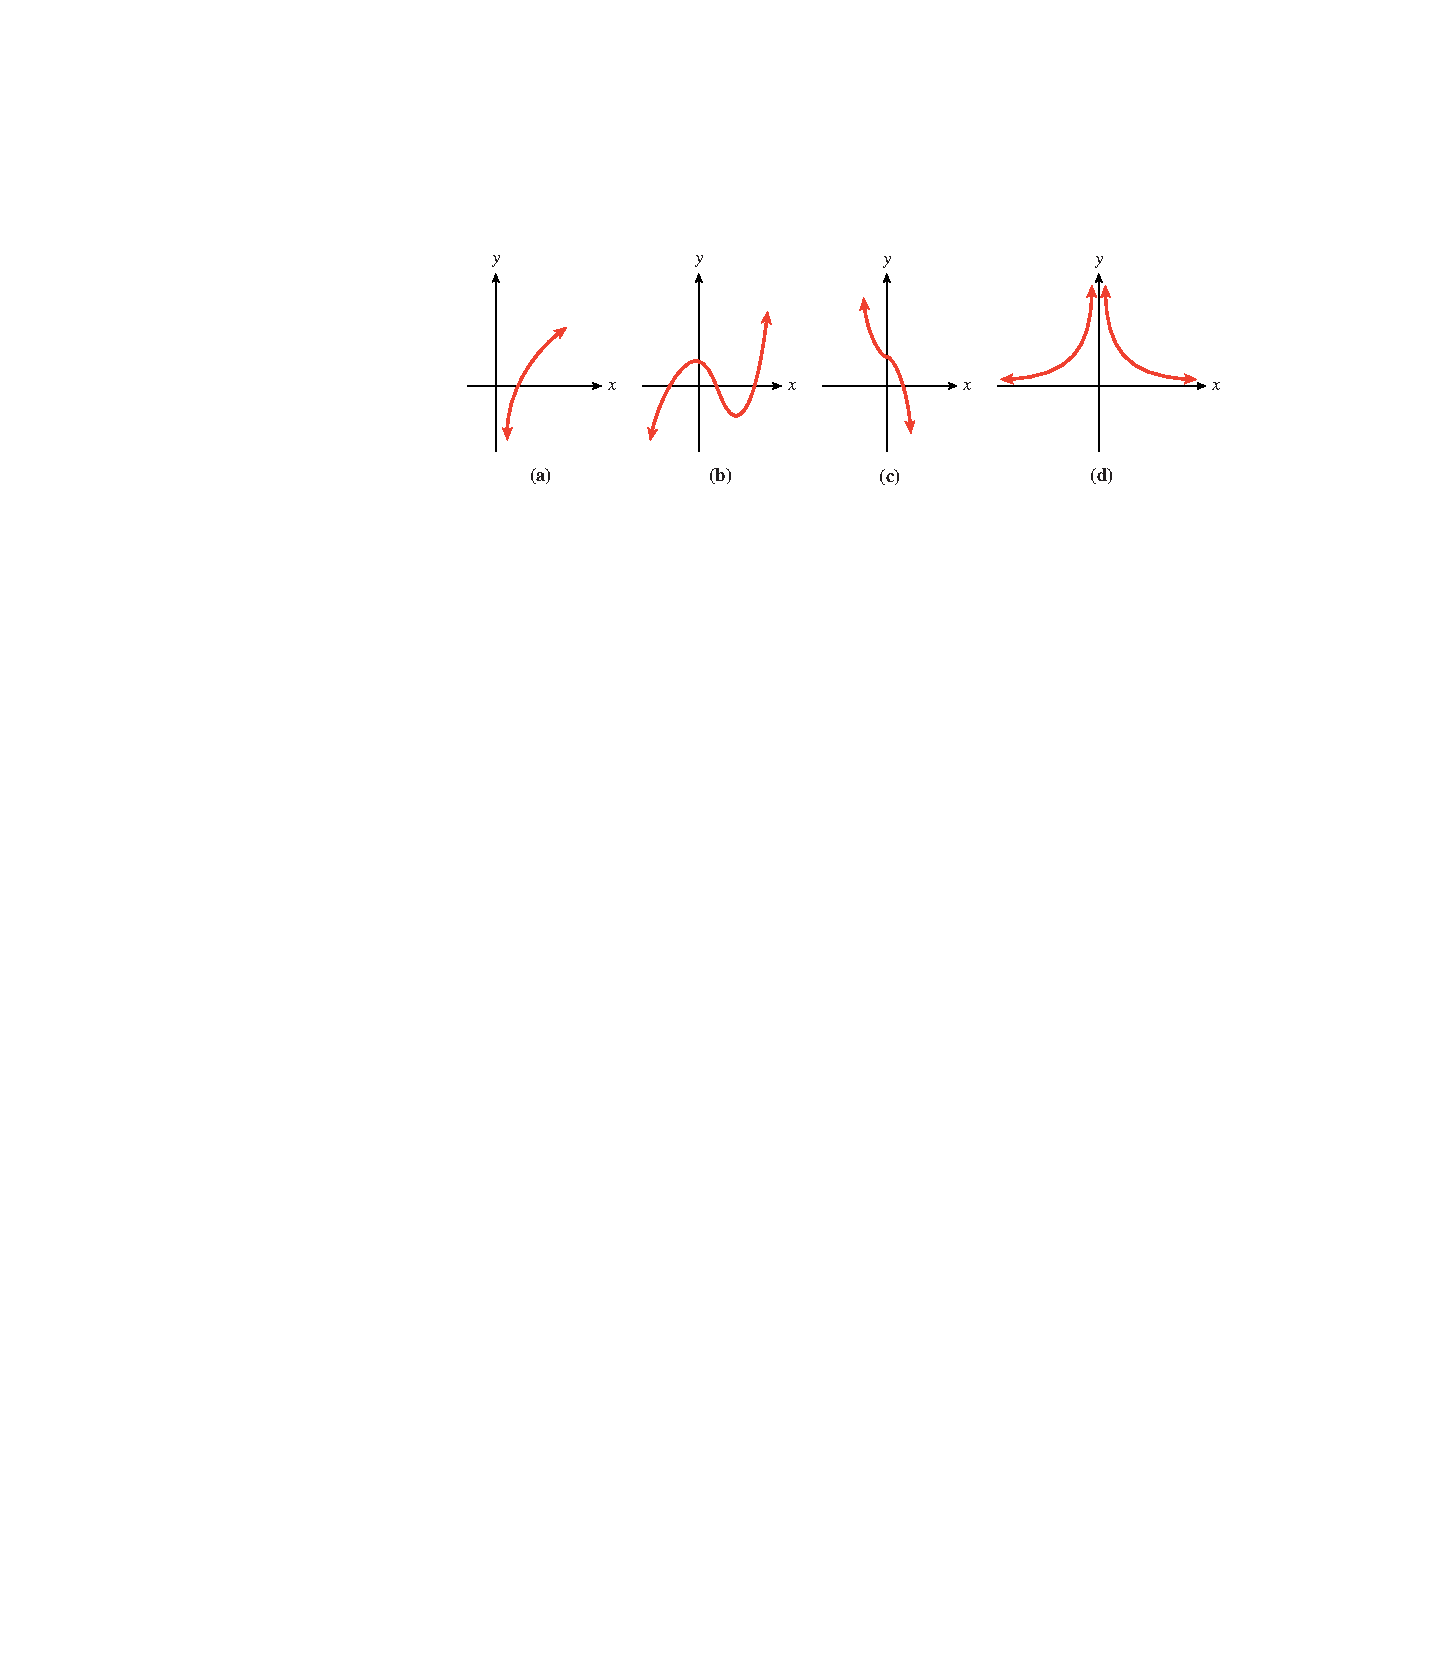
\includegraphics[width=0.9\linewidth]{images/fig-invertible-or-not}
\caption{\label{fig-invertible-or-not}}
\end{figure}
\par\smallskip%
\noindent\textbf{Solution.}\hypertarget{solution-9}{}\quad%
\hypertarget{p-116}{}%
In each case, apply the horizontal line test to determine whether the function is invertible. Because no horizontal line intersects their graphs more than once, the functions pictured in \hyperref[fig-invertible-or-not]{Figures~\ref{fig-invertible-or-not}}(a) and (c) are invertible. The functions in \hyperref[fig-invertible-or-not]{Figures~\ref{fig-invertible-or-not}}(b) and (d) are not invertibe.%
\end{example}
\hypertarget{p-117}{}%
We have been talking about how to tell if the inverse of a function is also a function, but in practice this is not the language typicaly used. Usually we ask this same question in the form "Is the function invertible?" The following definition explains this relationship: \begin{assemblage}[Invertible Function]\label{assemblage-18}
\hypertarget{p-118}{}%
If \(y=f(x) \) is a function such that its inverse, \(x=f^{-1}(y)\), is also a function then we say that \(f(x) \) is an \terminology{invertible function}.%
\end{assemblage}
%
\par
\hypertarget{p-119}{}%
The inverse function \(f^{-1}\) undoes the effect of the function \(f\). The function \(f(t) = 6 + 2t\) multiplies the input by \(2\) and then adds \(6\) to the result. The inverse function \(f^{-1}(H) = \dfrac{H -6}{2}\) undoes those operations in reverse order: It subtracts \(6\) from the input and then divides the result by \(2\).%
\par
\hypertarget{p-120}{}%
If we apply the function \(f\) to a given input value and then apply the function \(f^{-1}\) to the output from \(f\), the end result will be the original input value. For example, if we choose \(t = 5\) as an input value, we find that \begin{align*} f(5)\amp= 6 + 2(5) = 16\amp\amp\text{ Multiply by 2, then add 6.}\\ \text{and } f^{-1}(16) \amp = \frac{16 - 6}{2} = 5.\amp\amp\text{Subtract 6, then divide by 2.} \end{align*}%
\begin{figure}
\centering
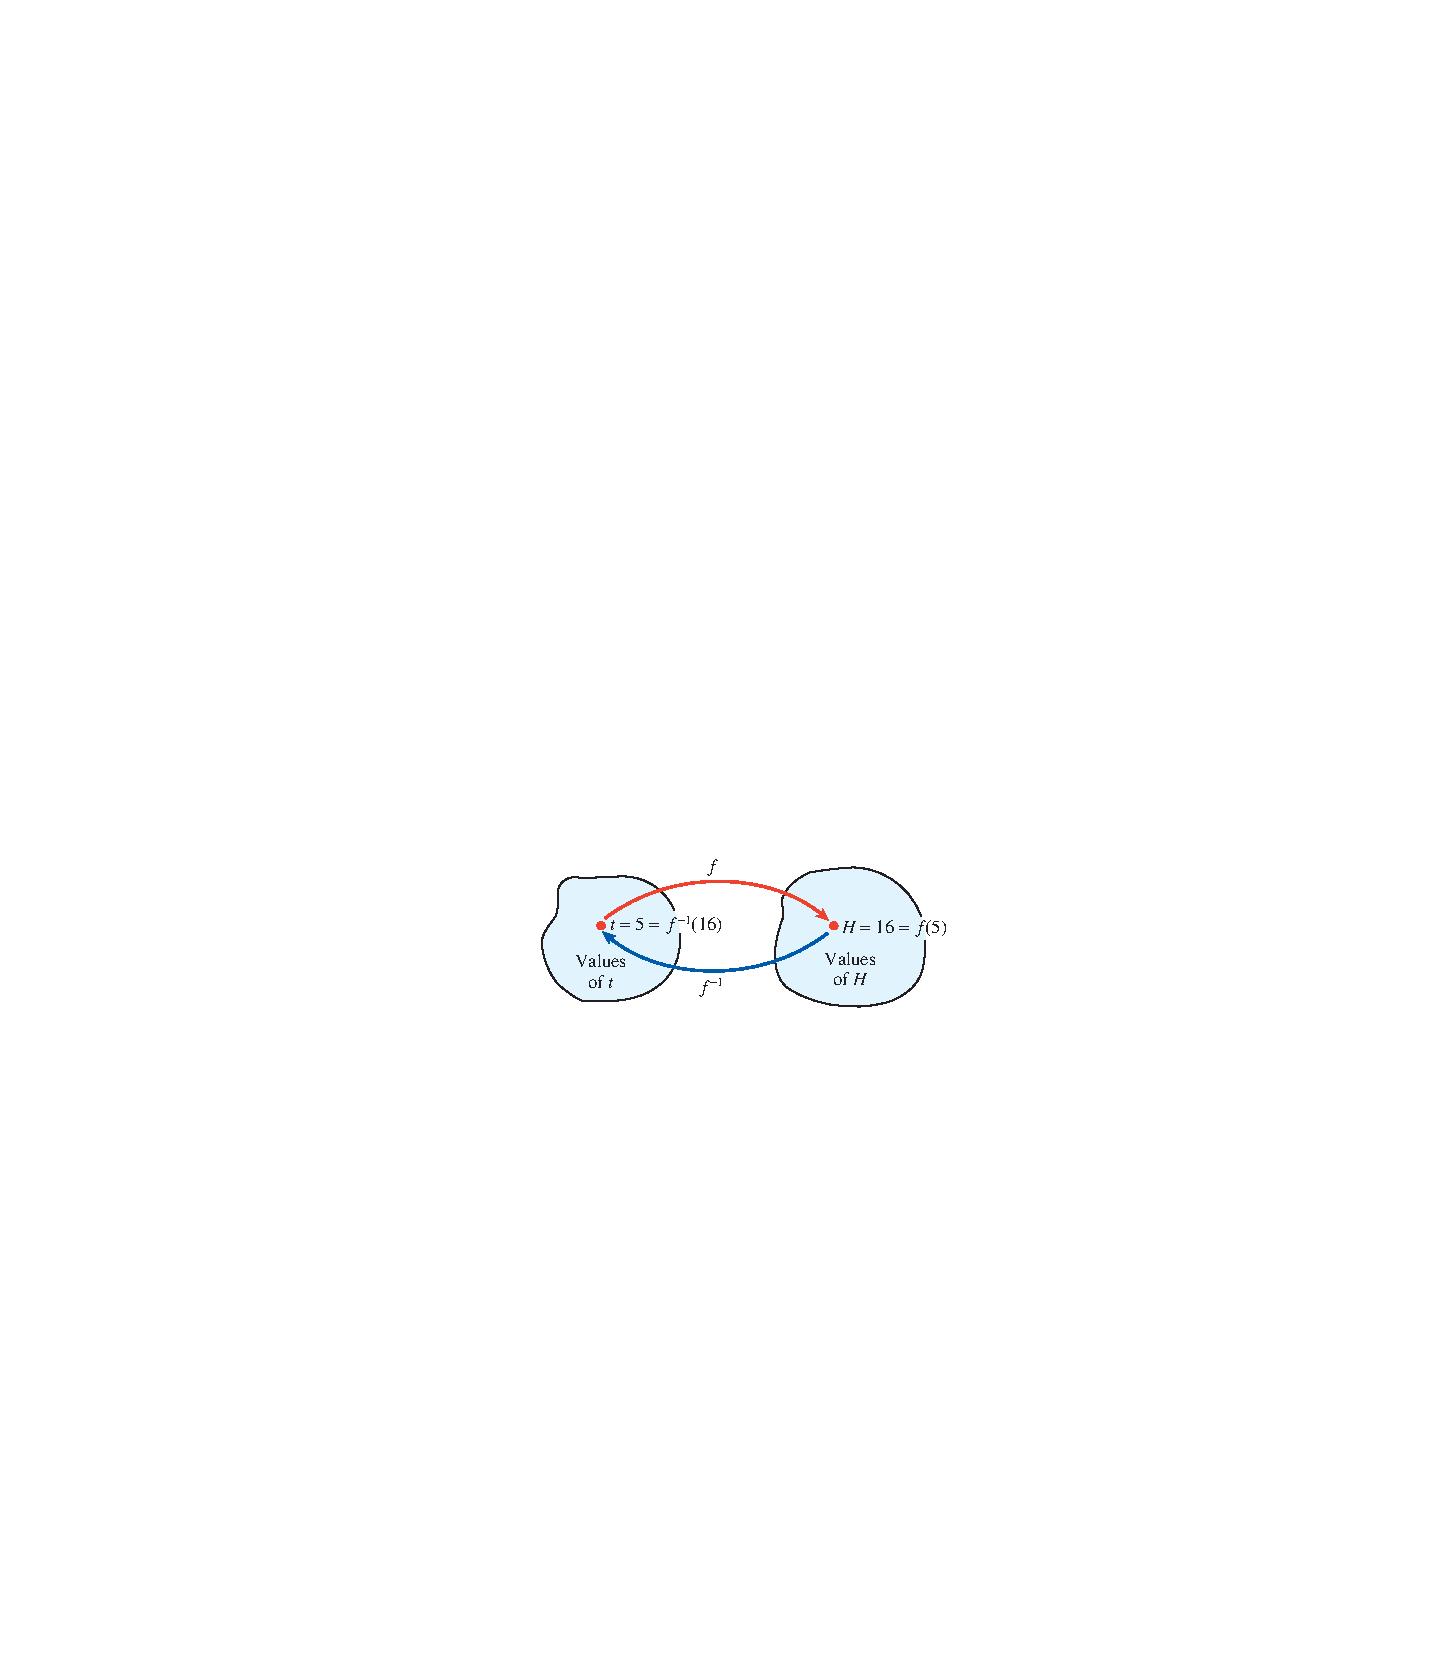
\includegraphics[width=0.5\linewidth]{https://mathbooks.unl.edu/PreCalculus/images/fig-function-and-inverse-diagram.pdf}
\caption{\label{fig-function-and-inverse-diagram}}
\end{figure}
\hypertarget{p-121}{}%
We return to the original input value, \(5\).%
\typeout{************************************************}
\typeout{Exercises 1.11 Exercises}
\typeout{************************************************}
\section[{Exercises}]{Exercises}\label{exercises-1}
\begin{exerciselist}
\item[1.]\hypertarget{exercise-1}{}(Slope and Intercept)\space\space{}